\documentclass[11pt, oneside]{Thesis} % The default font size and one-sided printing (no margin offsets)

\graphicspath{{Figures/}} % Specifies the directory where pictures are stored

\usepackage{natbib} % Use the natbib reference package - read up on this to edit the reference style; if you want text (e.g. Smith et al., 2012) for the in-text references (instead of numbers), remove 'numbers' 
\usepackage{mathptmx}
\usepackage{amsmath}
\usepackage{amssymb}
\usepackage{mathrsfs}
\usepackage{gensymb}
\usepackage{pdflscape}
\usepackage{pifont}
\usepackage{afterpage}
\usepackage{multirow}
\usepackage{paralist}

\hypersetup{urlcolor=black, colorlinks=true} % Colors hyperlinks in blue - change to black if annoying
\title{\ttitle} % Defines the thesis title - don't touch this

\begin{document}

\frontmatter % Use roman page numbering style (i, ii, iii, iv...) for the pre-content pages

\setstretch{1.3} % Line spacing of 1.3

% Define the page headers using the FancyHdr package and set up for one-sided printing
\fancyhead{} % Clears all page headers and footers
\rhead{\thepage} % Sets the right side header to show the page number
\lhead{} % Clears the left side page header

\pagestyle{fancy} % Finally, use the "fancy" page style to implement the FancyHdr headers

\newcommand{\HRule}{\rule{\linewidth}{0.5mm}} % New command to make the lines in the title page

% PDF meta-data
\hypersetup{pdftitle={\ttitle}}
\hypersetup{pdfsubject=\subjectname}
\hypersetup{pdfauthor=\authornames}
\hypersetup{pdfkeywords=\keywordnames}

%----------------------------------------------------------------------------------------
%	TITLE PAGE
%----------------------------------------------------------------------------------------

\begin{titlepage}
\begin{center}

\textsc{}\\[1.5cm] % University name
\textsc{}\\[0.5cm] % Thesis type

\textsc{}\\[0.4cm]
{\huge \bfseries \ttitle}\\[0.4cm] % Thesis title
\textsc{}\\[1.5cm]
 
\begin{minipage}{0.4\textwidth}
\begin{flushleft} \large
\emph{Author:}\\
{\authornames} % Author name - remove the \href bracket to remove the link
\end{flushleft}
\end{minipage}
\begin{minipage}{0.4\textwidth}
\begin{flushright} \large
\emph{Supervised by:} \\
{\supname} % Supervisor name - remove the \href bracket to remove the link  
\end{flushright}
\end{minipage}\\[3cm]


\groupname\\\deptname\\\univname\\[2cm] % Research group name and department name
\large \textit{Submitted to the University of Hertfordshire in partial fulfilment of the requirements of the degree of \degreename.}\\[0.3cm] % University requirement text
\textit{}\\[0.4cm]
 
{\large May 2016}\\[4cm] % Date
%\includegraphics{Logo} % University/department logo - uncomment to place it
 
\vfill
\end{center}

\end{titlepage}

\clearpage % Start a new page

%----------------------------------------------------------------------------------------
%	ABSTRACT PAGE
%----------------------------------------------------------------------------------------

\pagestyle{empty} % No headers or footers for the following pages

\addtotoc{Abstract} % Add the "Abstract" page entry to the Contents

\abstract{\addtocontents{toc}{\vspace{1em}} % Add a gap in the Contents, for aesthetics

In this {\paperorthesis} the stellar rotation signal for {\prox} is investigated. High-resolution spectra taken with
{\uves} and {\harps} of {\prox} over a 13-year period is used as well as photometric observations of {\prox} from
{\asas} and {\hst}.

The {\ha} equivalent width and {\ha} index are measured (and found to be very similar), together with other measurements,
  skewness and kurtosis and a method that investigates the symmetry of the line, the Peak Ratio, is introduced which
  appears to return better results than the other measurements.

The investigations return a most significant period of \examrevision{82.6 $\pm$ 0.1} days, confirming photometric
  results and ruling out a more recent result of 116.6 days which it is concluded is an artefact of the observation
  times.

It is also concluded that whilst spectroscopic {\ha} measurements can be used for period recovery, in the case of
   {\prox} the available photometric measurements are more reliable.  By using 2D models of {\prox} to generate
   simulated {\ha}, it is found that reasonable distributions of plage and chromospheric features are able to reproduce
   the equivalent width variations in observed data and recover the rotation period. \examrevision{The period recovery
   is still effective after simulated noise and the effects of flares similar to those in the observed data the are
   added to the modelling results. However the 2D models used fail to generate the observed variety of line shapes
   measured by the peak ratio. It is concluded that only 3D models which incorporate vertical motions in the
   chromosphere can achieve this.}

}

\clearpage % Start a new page


%----------------------------------------------------------------------------------------
%	DECLARATION
%----------------------------------------------------------------------------------------

\setstretch{1.3} % Reset the line-spacing to 1.3 for body text (if it has changed)

\Declaration{ % Add a gap in the Contents, for aesthetics

% See sections 15.5 -- 15.7 of the regulations for research students
  
I declare that no part of this work is being submitted concurrently
for another award of the University or any other awarding body or
institution. This thesis contains a substantial body of work that has
not previously been submitted successfully for an award of the
University or any other awarding body or institution.

Except where indicated otherwise in the submission, the submission is
my own work and has not previously been submitted successfully for any
award.
}
\clearpage % Start a new page


%----------------------------------------------------------------------------------------
%	ACKNOWLEDGEMENTS
%----------------------------------------------------------------------------------------

\setstretch{1.3} % Reset the line-spacing to 1.3 for body text (if it has changed)

\acknowledgements{\addtocontents{toc}{\vspace{1em}} % Add a gap in the Contents, for aesthetics

{\FirstP} gratefully acknowledge the advice and assistance of members of the Centre for Astrophysical Research at the
University of Hertfordshire in the preparation of this {\paperorthesis}.  \IfThesis{I particularly want to thank my
  supervisors, Prof. H.R.A. Jones and Dr J. R. Barnes, originally at the University of Hertfordshire and the latter now
  at the Open University for their advice and assistance, particularly in bringing me up to speed in things I hadn't
  learnt properly (or at all) 4 decades ago.}

The {\harps} data was obtained from HARPS public database at the European Southern Observatory (ESO).

{\FirstP} also wish to thank Birgit Fuhrmeister and Lalitha Sairam for providing {\Firstobj} with some additional data
referred to in \citet{fuhrmeister11}.

{\FirstP} acknowledge the value of the Vienna Atomic Line Database (VALD) for spectral line data and the {\asas} for
additional observations of {\prox}.

All the figures were produced using \matplot, which is associated with the {\scipy} library \citep{jones01}.

Finally \PaperThesis{the lead author}{I} must express \IfThesis{my}\IfPaper{his} thanks to \PaperThesis{his}{my} wife,
Sue Collins, for proof-reading and tolerating for most of the time \IfPaper{his}\IfThesis{my} absence or distracted
attention during the preparation of this \paperorthesis.

}
\clearpage % Start a new page
%----------------------------------------------------------------------------------------
%	LIST OF CONTENTS/FIGURES/TABLES PAGES
%----------------------------------------------------------------------------------------

\pagestyle{fancy} % The page style headers have been "empty" all this time, now use the "fancy" headers as defined before to bring them back

\lhead{\emph{Contents}} % Set the left side page header to "Contents"
\tableofcontents % Write out the Table of Contents

\lhead{\emph{List of Figures}} % Set the left side page header to "List of Figures"
\listoffigures % Write out the List of Figures

\lhead{\emph{List of Tables}} % Set the left side page header to "List of Tables"
\listoftables % Write out the List of Tables

%----------------------------------------------------------------------------------------
%	ABBREVIATIONS
%----------------------------------------------------------------------------------------
% COMMENT OUT THIS SECTION IF YOU DON'T WANT TO INCLUDE ABBREVIATIONS

\clearpage % Start a new page

\setstretch{1.5} % Set the line spacing to 1.5, this makes the following tables easier to read

\lhead{\emph{List of Abbreviations}} % Set the left side page header to "Abbreviations"
\listofsymbols{ll} % Include a list of Abbreviations (a table of two columns)
{
\textbf{ASAS} & \textbf{A}ll \textbf{S}ky \textbf{A}utomated \textbf{S}urvey \\
\textbf{FAP} & \textbf{F}alse \textbf{A}larm \textbf{P}robability \\
\textbf{HARPS} & \textbf{H}igh \textbf{A}ccuracy \textbf{R}adial velocity \textbf{P}lanet \textbf{S}earcher \\
\textbf{UVES} & \textbf{U}ltraviolet and \textbf{V}isual \textbf{E}chelle \textbf{S}pectrograph \\
}

%----------------------------------------------------------------------------------------
%	THESIS CONTENT - CHAPTERS
%----------------------------------------------------------------------------------------

\mainmatter % Begin numeric (1,2,3...) page numbering

\pagestyle{fancy} % Return the page headers back to the "fancy" style

% Include the chapters of the thesis as separate files from the Chapters folder
% Uncomment the lines as you write the chapters

\chapter{Introduction}
\protect\label{chapter:introduction}
\lhead{Chapter \ref{chapter:introduction} . \emph{Introduction}}

\section{The importance of the study of {\rdwarf} stars}
\protect\label{section:introrwarfs}

{\rdwarf} stars are particularly important as a field of study. One major reason for this is that they account for over
75\% of the stars within 25 pc of the Sun, as described in \citet{winters15}. Indeed our nearest neighbour, \prox, is an
M5.5V star. Studies such as \citet{vandokkum2010} have argued for a similar proportion of {\rdwarf} stars in galaxies
other than the Milky Way, although that paper concedes the impossibility of observing them individually
\examrevision{as, for example,} a star such as Barnard's star with an absolute magnitude of about 13 would have a K band
magnitude of about 39 at the distance of the Virgo cluster. The stellar populations of other galaxies is a field of
considerable interest in itself, but one well outside the scope of this \paperorthesis.

\examrevision{{\rdwarf} stars are also of great interest in the search for exoplanets. Having lower mass than earlier
  type stars, the radial velocity variations induced by planetary orbits is proportionally greater. In
  \citet{johnson07}, it is seen that the likelihood of planets approaching Earth-size is actually higher than for G or K
  stars and in \citet{barnes12} a search for such planets in the habitable zone of \rdwarf s was undertaken. In both
  \citet{barnes14} and \citet{tuomi14} the likelihood of such planets in the habitable zone of \rdwarf s is discussed
  further. The habitable zone of the much cooler \rdwarf s would obviously be much closer to the stars than the Sun,
  less than 0.1 AU, with complications such as tidal locking of planets and their exposure to flares. Despite these
  drawbacks to habitability, the longevity of the much slower burning \rdwarf s by comparison with earlier spectral type
  stars would enhance the opportunities for biological evolution to take hold at some stage.}

\examrevision{In the search for the periodic signatures of exoplanets, it is obviously necessary to distinguish between
  those and the rotation period of the star itself. The orbital period of exoplanets of particular interest, as being
  potentially in the habitable zone close to an {\rdwarf}, is of the order of around 10 days, shorter than the 24-day
  rotation period of the sun. Also, as observed later in this \paperorthesis, aliases can arise from the combination of
  two or more different periods. This has been the focus of intensive debate in recent papers which have expressed quite
  divergent views regarding whether reported planets have been validly detected by their period such as in
  \citealt{barnes13,robertson14,robertson14a,tuomi13aug,robertson15}.}

\section{Activity and the rotation period}
\protect\label{section:introrotation}

Despite their abundance, many aspects of the activity of \rdwarf s have remained less well characterised
\examrevision{compared to other classes of star}, mainly because of their inherent faintness. Stars become fully
convective \examrevision{below} around M4V and the transition to this regime has been a subject of some study, as for
example the conference proceedings of \citet{stassun11}.

Of particular interest is the study of complex magnetic activity in such stars and consideration of the dynamo systems
which would give rise to this. Authors such as \citet{morin11} argue for two simultaneous dynamos, whereas
\citet{kitchatinov14} discount this and argue for some of the observed activity being due to magnetic field inversions.

In \citet{mohanty03} the authors set out the correlation between the \examrevision{projected} rotational velocity
{\vsini} and the activity in mid-M to L-dwarfs, \examrevision{charting} activity against rotational velocity up to about
12 km/s where a saturation velocity is observed. They also note an increase \examrevision{in} rotation velocities for
later stars and a drop-off in activity for \ldwarf s. This is developed further in \citet{reiners08} and also
\citet{schmidt14}, however the latter disagree with the previously-reported drop-off in activity for \ldwarf s, arguing
that dust affects the measurements of activity, \examrevision{reporting activity in \ldwarf s down to L6}.

In \citet{mohanty02} the relation between activity and rotational velocity is explored, however both in this and in
\citet{mohanty03} the authors state that the correlation between rotation and activity \examrevision{is not as strong in} 
fully convective stars from M3 on and suggest \examrevision{that a ``turbulent dynamo'' is responsible}.

It is clear that the measurement of rotational velocity is of importance for a full understanding of these processes.

\section{The importance of {\ha}}
\protect\label{section:intohalpha}

The {\ha} line is a powerful diagnostic tool in many areas of astronomy. For example, {\ha} luminosity is one of the key
ways of estimating the star formation rates in galaxies (see for example \citet{rosagonzalez02}).
In terms of the study of stars, since the core of {\ha} forms above the photosphere, as shown in \citet{vernazza81}, it
is an important line for studying activity and variability in stellar chromospheres \citep{hall08}. Chromospheric
features such as plage regions and jets are seen well in {\ha} (see for example \citet{kneer10} and \citet{kuridze11}).
The behaviour of the {\ha} line in {\rdwarf} stars is seen as a key diagnostic of activity, as shown in the
previously-cited papers (\citealt{mohanty02, mohanty03, reiners08, schmidt14}) which describe the relationship between
rotation and activity.

The behaviour of the {\ha} line is a potentially important diagnostic because it is sensitive to magnetic activity and
is a strong line usually seen in emission in later {\rdwarf} stars. It is used as the measure of activity in, for
example \citet{mohanty03} and subsequent papers. In \citet{hatzes15} the {\ha} periodicity is explicitly studied in
relation to \examrevision{GL 581 and whether the exoplanet GL 581d is indeed real or is actually an alias, which has
  been debated extensively in \citealt{barnes13,robertson14,tuomi13aug,robertson15a}}.

This {\paperorthesis} investigates whether periodicity can be identified in the morphology of the {\ha} line obtainable
from high-resolution spectra such as those obtained from the \textit{Ultraviolet and Visual Echelle Spectrograph}
({\uves}) at the 8.2m Very Large Telescope (VLT, UT 2) and the \textit{High Accuracy Radial velocity Planet Searcher}
({\harps}) at the ESO La Silla 3.6m telescope. \citet{barnes14} noticed that while a strong transient emission in {\ha}
was observable during flares, \examrevision{it should nevertheless be possible to derive periodicity from the morphology
  of the {\ha} line. On the other hand, it must be said} that in \citet{reiners09}, the authors suggest that Ca, He and
{\ha} lines, being chromospheric emissions, are strongly affected by activity and should be omitted when searching for
radial velocities in active \rdwarf s.

Conscious of these divergent views, this {\paperorthesis} attempts to study the merits of precision measurements using
chromospheric features and in particular {\ha} analysis.

\section{\prox}
\protect\label{section:introprox}

As the nearest star to the solar system at a distance of 1.3 parsecs, {\prox} is a bright M5.5V star with a magnitude of
11.13 in the V-band and is of obvious interest with extensive data sets available. The {\ha} line is always in emission
with a characteristic shape. Thus is it a good place to test the general methodology applicable to late \rdwarf s.

\examrevision{{\prox} is part of a system of three stars together with Alpha Centauri A and B and of higher metallicity
  than the Sun, as described in \citet{linsky04}. This further focuses interest on the search for rocky planets and ones
  to be found in the habitable zones of those stars, with one recently discovered for {\prox} and reported in
  \citet{angladaescude16}.}

Despite the interest and available data, the rotation period of {\prox} is nevertheless uncertain.  Previous studies
have reported periods ranging from the $ 31.5 \pm 1.5 $ days of \citet{guinan96}, the 41.3 days of \citet{benedict93}
and s between 82 and 84 days in \citealt{benedict92,benedict98}.  \citet{kurster99} found that the period is not less
than 50 days, \examrevision{whilst more recently \citet{kiraga07} reported a value of 82.5 days}. \examrevision{All these
  estimates were based on photometric measurements}.  In \citet{cincunegui07} a 447-day activity cycle is reported,
based upon {\ha} measurements. Latterly \citet[Table 3]{suarezmascareno15} reported a value of 116.6 days, again using a
measurement of {\ha}.

{\prox} has quite frequent flares \examrevision{and whilst they obviously disturb the measurements, they enable a study
  to be made of and to what extent they compromise} methods for the calculation of the rotation period.

\section{Methodology}
\protect\label{section:methodology}

The approach taken in this {\paperorthesis} is as follows \examrevision{is similar} to that taken \examrevision{by}
\citet{giguere16} for the K dwarf $\epsilon$ Eridani. In Chapter \ref{chapter:photometry} photometric measurements of
\examrevision{the} periodicity \examrevision{of} {\prox} are examined, as these prove a useful benchmark for
spectroscopic measurements. In Chapter \ref{chapter:proxima} the measurement methods are introduced which are
subsequently used to investigate periodicity from sets of spectra. In Chapter \ref{chapter:modelling} possible models of
{\prox} are studied and attempts \examrevision{are} made to apply the measurement methods to simulated spectra to evaluate their
performance, obtain error estimates and determine how \examrevision{these vary} with poorer signal to noise ratio. Chapter
\ref{chapter:discussion} and \ref{chapter:conclusions} report the discussion and conclusions of this study. Appendices
describe some of the software tools developed and used and list \examrevision{some additional results}.

\chapter{Periodicity from photometric measurements} % Main chapter title
\protect\label{chapter:photometry}
\lhead{Chapter \ref{chapter:photometry}. \emph{Periodicity of {\prox} from photometric measurements}}

To process the data for all the periodicity studies in this \paperorthesis, all but one item\footnote{The {\numrecs}
  Lomb-Scargle program, the Fortran version of which was modified and used.} of the associated software was written in
Python using the Lomb-Scargle routines described in Appendix \ref{chapter:lsroutines}.

As nearly all previous measurements of periodicity in {\prox} were made using Photometric observations, in this
{\paperorthesis}, before discussing spectroscopic measurements such as with the {\harps} data and the various methods of
analysing the {\ha} lines, some photometric observations for {\prox} are considered.

\section{ASAS}
\protect\label{section:asas}

First is presented results obtained from the Photometric observations for {\prox} taken from the V-Band (there were no
data for the I-Band) of the All Sky Automated Survey (\asas), \citep{pojmanski97}, which contains data between the
periods December 2000 to September 2009.

As indicated by the {\asas} guidelines\footnote{This is described in http://www.astrouw.edu.pl/asas/explanations.html},
with {\prox} having magnitude 11 in the V-band, the data was taken from the second aperture. Initially only the ``best''
(grade A) data from this aperture is considered, which has 970 points. Obtaining a periodogram from this, using the
{\numrecs} routine, which returns False Alarm Probabilities, the periodogram shown in Fig. \ref{fig:asaspgram1} is
obtained, restricting the display from 20 to 160 days.

\begin{figure}[!htbp]
\begin{center}
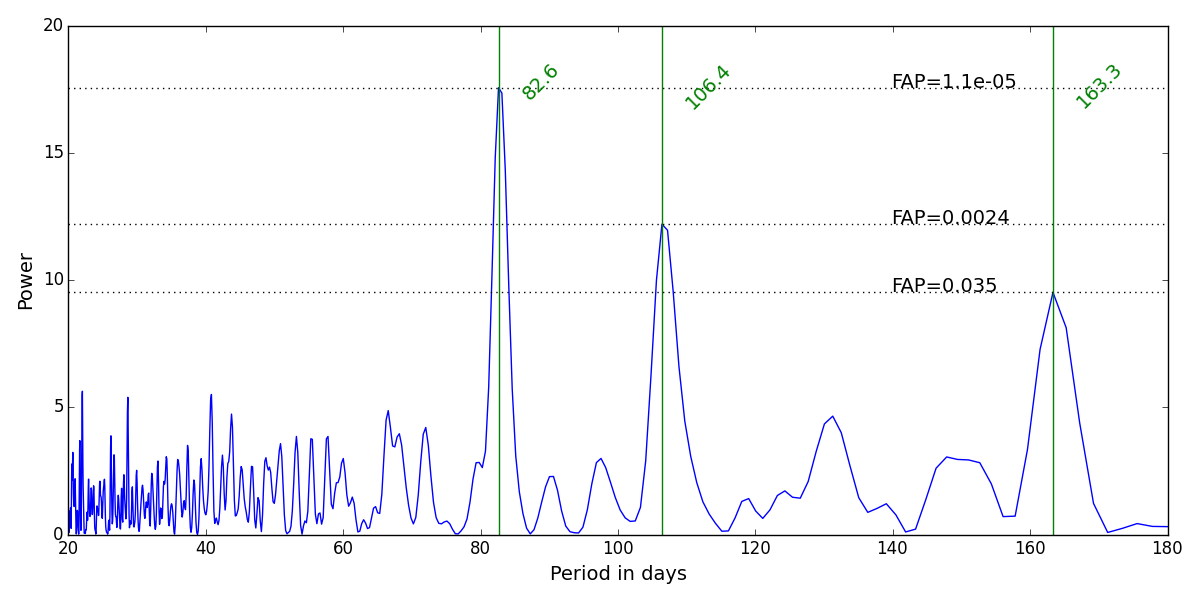
\includegraphics[scale=0.30]{Figures/asasnobin.png} \\
\end{center}
\caption{This is a periodogram from the {\asas} database for {\prox} second aperture, without binning, containing 970
  points, considering only periods between 20 and 160 days.}
\protect\label{fig:asaspgram1}
\end{figure}

\begin{figure}[!htbp]
\begin{center}
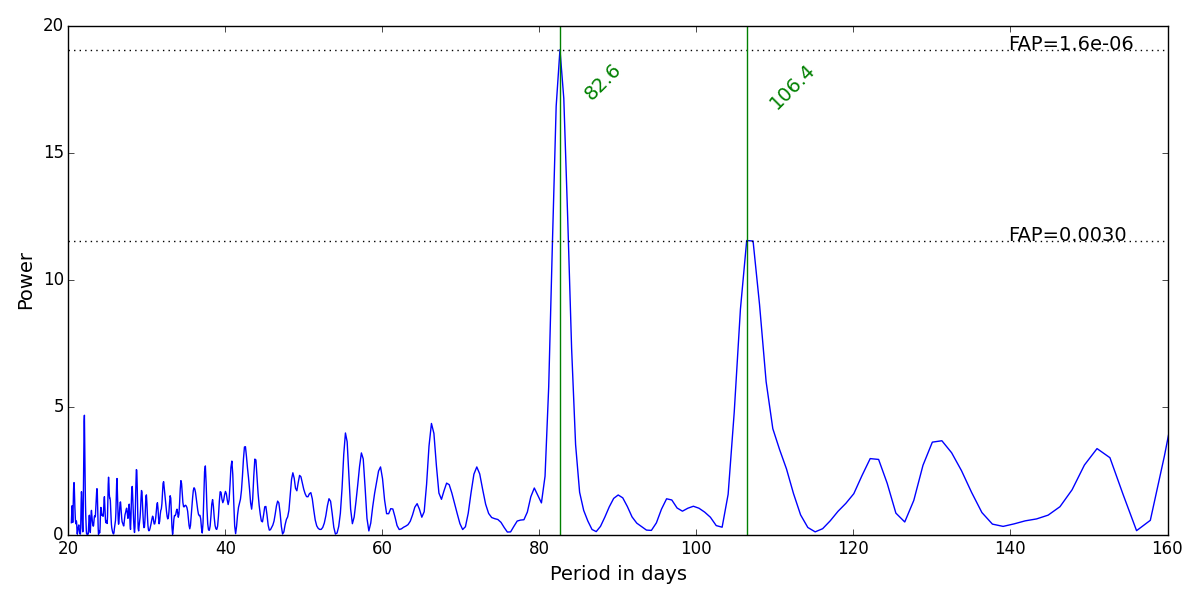
\includegraphics[scale=0.30]{Figures/asasbin1.png} \\
\end{center}
\caption{This is a periodogram from the {\asas} database for {\prox} second aperture, binned to 1 day, containing 624 points.}
\protect\label{fig:asaspgram2}
\end{figure}

\begin{figure}[!htbp]
\begin{center}
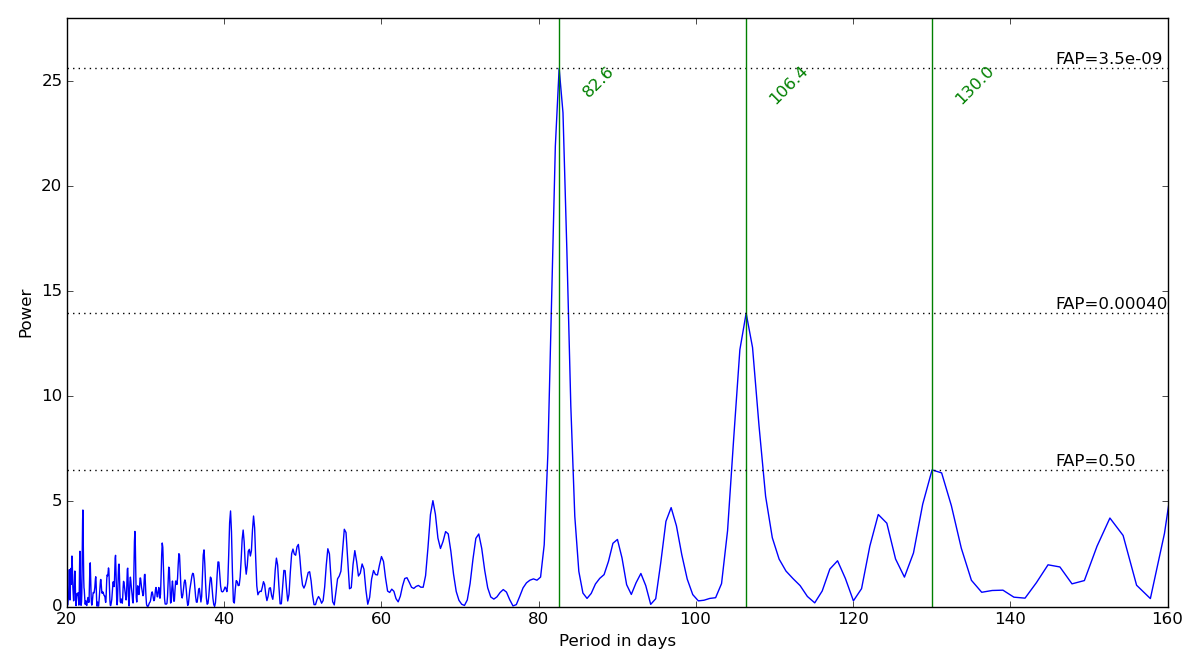
\includegraphics[scale=0.30]{Figures/asasbin18min.png} \\
\end{center}
\caption{This is a periodogram from the {\asas} database for {\prox} second aperture, binned to 18 minutes, containing 924 points.}
\protect\label{fig:asaspgram3}
\end{figure}

As some of the observations were duplicated or apparently overlapping, these were initially binned to 1 day, in line
with several of the {\harps} results described in Section \ref{section:harpsper}. This reduced the number of points to
624. From the result the periodogram shown in Fig. \ref{fig:asaspgram2} was obtained. This appeared to clarify the peaks
by reducing the number with very short periods and enhancing the two major ones. Some binning appeared to be necessary
as some of the points had duplicated times. It appeared worthwhile to experiment with sizes of binning to see at what
point the result was optimal, in terms of yielding the strongest peaks with the lowest FAP and least extraneous peaks
and after trying various binning values between several days down to 1 minute, the optimal binning was found to be 18
minutes, yielding the periodogram shown in Fig. \ref{fig:asaspgram3}. Note that the scale of this is the same but the
figure has been made taller to accommodate the more powerful 82.6 day peak. The reduction of the points in the binning to
18 minutes was found to be a much more modest reduction, to 924 observations from 970.

The explanation of this 18-minute binning result may be related to the 3-minute exposure time for {\asas} 3
\citep{pojmanski01}. Possibly this may also be related to a p-mode oscillation of \prox, however no current results are
available for this in the literature.

Although the recommended aperture by {\asas} for {\prox} is the second aperture, it appeared valuable to compare the
three highest peaks from each of the apertures finding that nearly all the data gave a first peak of 82.6 days, a second
peak of 106.4 days and a much smaller third peak of about 131 days in most cases. The results are listed with
no-binning, 1-day and 18-minute binnings in Table \ref{table:asasperiods}. Also considered were the other grades of
{\asas} data, mostly from ID 142944-6241.0, with a little under half of the Class A Data, 416 points and much higher
error rating. All the periodograms from this lower quality data still showed a strong peak of around 82.5 days. The
results for 18-minute binning are shown in Table \ref{table:lqasas}.

\begin{table}[!htbp]
\centering
\scalebox{0.8}{
\begin{tabular}{|l|l|r|r|r|}
\hline
Aperture & binning & Peak 1 & Peak 2 & Peak 3 \\\hline
1 & none & 83.1 & 106.4 & 131.3 \\
2 & none & 82.6 & 106.4 & 22.0 \\
3 & none & 82.6 & 106.4 & 131.3 \\
4 & none & 82.6 & 106.4 & 131.3 \\
5 & none & 82.6 & 106.4 & 131.3 \\\hline
1 & 1 day & 82.6 & 106.4 & 110.6 \\
2 & 1 day & 82.6 & 106.4 & 22.0 \\
3 & 1 day & 82.6 & 106.4 & 130.0 \\
4 & 1 day & 82.6 & 106.4 & 42.6 \\
5 & 1 day & 82.6 & 106.4 & 42.4 \\\hline
1 & 18 min & 83.1 & 106.4 & 131.3 \\
2 & 18 min & 82.6 & 106.4 & 130.0 \\
3 & 18 min & 82.6 & 106.4 & 130.0 \\
4 & 18 min & 82.6 & 106.4 & 130.0 \\
5 & 18 min & 82.6 & 106.4 & 131.3 \\\hline
\end{tabular}}
\caption{Summary of three strongest periods taken from Class A values in {\asas} dataset for {\prox} from all apertures based upon magnitudes measured
  between December 2000 and September 2009. Results are shown for the raw data. 1-day binning and 18-minute binning.}
\protect\label{table:asasperiods}
\end{table}

\begin{table}[!htbp]
\centering
\scalebox{0.75}{
\begin{tabular}{|l|r|l|r|l|r|l|}
\hline
Aperture & Peak 1 & FAP & Peak 2 & FAP & Peak 3 & FAP \\\hline
1 & 83.1 & 0.0067 & 105.8 & 0.33 & 127.4 & 0.82 \\
2 & 83.1 & 0.03 & 105.8 & 0.43 & 127.4 & 0.61 \\
3 & 83.1 & 0.038 & 105.8 & 0.31 & 128.7 & 0.89 \\
4 & 84.1 & 0.1 & 105.8 & 0.21 & 128.7 & 0.93 \\
5 & 84.1 & 0.0024 & 105.8 & 0.0028 & 82.5 & 0.0033 \\\hline
\end{tabular}}
\caption{Summary of three strongest periods taken from Class B and lower quality values in {\asas} datasets for {\prox}
  based upon magnitudes measured between December 2000 and September 2009 binned to 18 minutes.}
\protect\label{table:lqasas}
\end{table}

It was noticeable that all of the Lomb-Scargle routines listed in Appendix \ref{chapter:lsroutines} gave exactly
the same results (apart from differences to scaling of the power) with all the {\asas} data, including the lower quality
data. This was in contrast to the Spectroscopic results discussed in later chapters of this \paperorthesis.

A search was made for very long periods up to the period spanned by the data in each case, however no strong periods
could be found, in particular nothing close to the 442 days reported in \citet{cincunegui07}.

\section{HST}
\protect\label{section:hst}

As another source of photometric results. periodograms were derived from the  {\hst} data discussed in
\citealt{benedict92,benedict98} consisting of 171 points obtained between July 1995 and January 1998, later enhanced so
the last 18 points extended to January 2001, Three times were actually duplicated and eliminating the duplications, it
was possible to obtain the periodogram in Fig. \ref{fig:hstb4min}.

\begin{figure}[!htbp]
\begin{center}
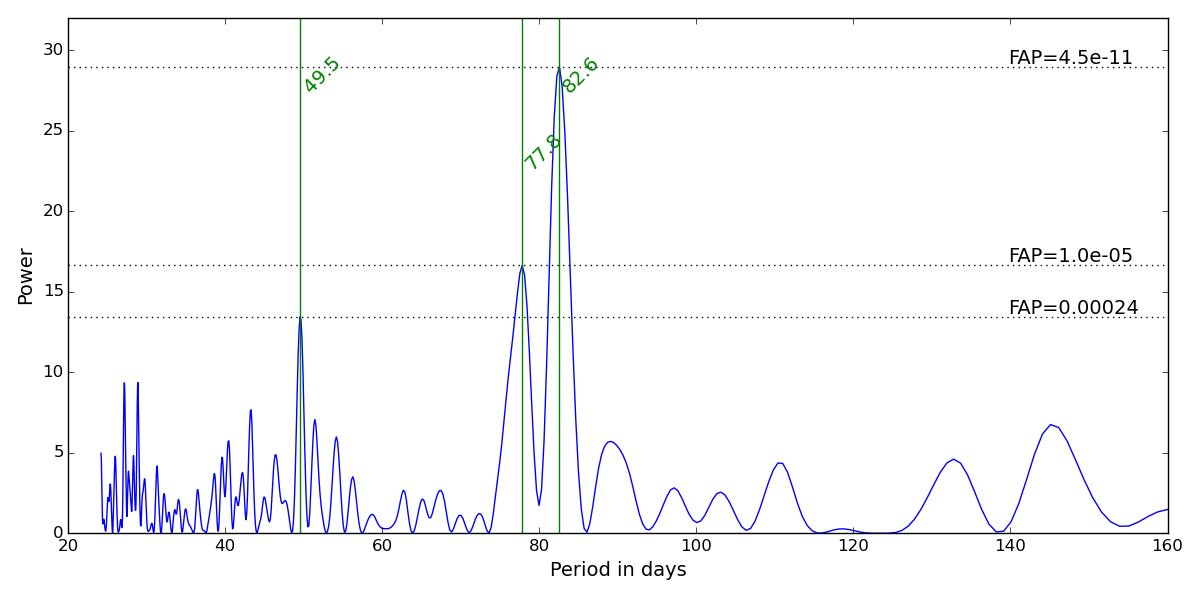
\includegraphics[scale=0.50]{Figures/hstb4min.png} \\
\end{center}
\caption{This is a periodogram from the {\hst} data discussed in \citet{benedict98} between July 1995 and January 1998 plus some additional
  points up to January 2001 examining periods showing the three highest peaks and with the FAPs marked in.}
\protect\label{fig:hstb4min}
\end{figure}

Again, as with the {\asas} data, all the Lomb-Scargle routines listed in Appendix \ref{chapter:lsroutines} gave exactly
the same results (other than the scaling of the power).

\section{Summary of photometric results}
\protect\label{section:summphotometric}

The period at 82.6 days is clearly as a strong, very low-FAP peak in both the {\asas} and {\hst} data. It is almost
certainly the rotation period of {\prox}, seemingly with a small error bar, although some investigations in Section
\ref{section:asasfap} were undertaken partly to investigate this.

It also provides a convenient benchmark for assessing the accuracy and reliability of the other, less clear
Spectroscopic methods investigated in Chapter \ref{chapter:proxima} based on the {\ha} line.

The {\asas} data, including the lesser quality data also included a strong peak at 106.4 days but this was not seen on
the {\hst} data. The former, however, has observation times much more constrained by the time of year and it is
noticeable that:

\begin{center}

$ \frac{1}{\frac{1}{82.6} - \frac{1}{365.25}} = 106.7 $

\end{center}

There remains the strong 77.8-day period seen in the {\hst} data but not in the {\asas} data to be accounted for,
possibly this period is a similar alias thrown up by the observation times as suggested for the 106-day period of
{\asas} data.


\chapter{Spectra of \prox}
\protect\label{chapter:proxima}
\lhead{Chapter \ref{chapter:proxima}. \emph{Spectra of \prox}}

Two sources of spectra for {\prox} are considered in this study, those from {\uves} taken between 10 and 14 March 2009
studied in \citet{fuhrmeister11} and {\harps} spectra with 260 data points between May 2004 and January 2014 from the
ESO archive\footnote{Based on data obtained from the ESO Science Archive Facility from programs 072.C-0488(E),
  082.C-0718(B), 183.C-0437(A) and 191.C-0505(A).} and referenced in \citet[Table 3]{suarezmascareno15}. The latter were
supplemented with 56 additional spectra from {\harps} taken between 19 January and 30 March 2016\footnote{Based on data obtained
  from the ESO Science Archive Facility from programs 096.C-0082(A) through to 096.C-0082(F).}. The {\uves} data were
obtained with a 0.8/1.10'' slit, yielding a resolution of approximately 60,000., while the resolution of {\harps} is
approximately 120,000. Also studied in Section \ref{section:uvesflares} are the X-ray data from XMM-Newton used in the
\citet{fuhrmeister11} paper\footnote{Provided by Fuhrmeister, priv. comm.} to identify any association between strong
X-ray values and possible corresponding changes to the {\ha} profile.

The bulk of the results from {\harps} in this chapter are taken using the full set of data up to 30 March 2016. However
reference is made to the original set to January 2014 (``Set to 2014'') as this is necessary to reproduce previous
calculations of the rotation period of \prox, in particular the 116.6 days reported by \citet[Table 3]{suarezmascareno15},
 which is not reproducible from the full set. The observation times in the Set to 2014 are used in the modelling results
in Chapter \ref{chapter:modelling} as nearly all the work on the modelling was completed prior to 2016.

\section{{\harps} and {\uves} spectra of \prox}

As mentioned in \citet{mohanty03} and subsequent papers such as \citet{jenkins09} and \citet{barnes14} the spectra of
the later of late \rdwarf s from approximately M5 onward, usually show {\ha} in emission, Several of the \rdwarf s
illustrated in \citet[Fig. 6]{barnes14} additionally show a distinct ``horned'' appearance, due to a certain amount of
self-absorption affecting the centre of the {\ha} peak. {\prox} consistently shows this pattern, which is displayed in
\citet[fig. 14]{fuhrmeister11}. The two \horn s surround a local minimum. As well as the equivalent width of the entire
{\ha} peak, the two \horn s vary in relative size over time on either side of the local minimum, which does not greatly
change in morphology over time. This would appear to be because a more symmetrically-distributed spectral line from the
photosphere is overlaid with plage and chromospheric effects which are asymmetric or localised to regions. These may be
compared with the H, K and Ca II lines discussed in \citet{rauscher06}. The main aim of this {\paperorthesis} is to
study the variations in the line and \horn s via various methods to see if periodicity may be reliably recovered.

\section{{\ha} Line measurements}
\protect\label{section:linemeas}

In Fig. \ref{fig:harpsfirstha}, on the left panel, are shown two example spectra from {\harps} nearly 2 years apart,
clearly showing the changes in the amplitude and shape of the {\ha} line. Fig. \ref{fig:harpsfirstha} also illustrates
the regions used to investigate periodic variability.

The spectra were first normalised by iteratively fitting a cubic polynomial to all the points in all the spectra, apart
from the {\ha} region, then excluding points outside 2 standard deviations above or below the fitted polynomial to
eliminate both emission and absorption lines. With the normalised spectra, the Equivalent Widths, abbreviated to ``EW''
hereafter are calculated. Also calculated is what is herein called the ``Peak Ratio'', abbreviated to ``PR'', defined as
the ratio of the mean values of the two \horn s. The ratio tabulated below is the mean value of the ``red'' \horn, i.e. that
for the longer wavelength, divided by the mean value of the ``blue'' {\horn} (i.e. the ratio of the longer wavelength to
the shorter wavelength \horn). For calculation of the Equivalent Width, values of the flux are interpolated up to the
boundaries of the regions chosen, to minimise integer pixel noise effects. The number of pixels in the regions, as
highlighted in Fig. \ref{fig:harpsfirstha} are either 35 or 36 for the {\ha} region and 11 or 12 for the red {\horn} and
14 or 15 for the blue {\horn} on {\uves}. The corresponding numbers on {\harps} are 98 or 99, 26 or 27 and 27 or 28
respectively. (The number of pixels could vary by one due to differing wavelength corrections caused by the heliocentric
component of the Radial Velocities.)

The {\ha} region for calculation of the Equivalent Width is set to encompass the {\ha} peak and runs from 6561.917{\AA}
to 6563.839\AA) as delineated by the dark red vertical lines. The regions selected for the blue and red \horn s are
shaded in blue and red and run from 6562.072{\AA} to 6562.613{\AA} and 6563.000{\AA} to 6563.517{\AA}
respectively. These regions were chosen to optimise variability in the line profiles. Note that the regions selected for
calculation of the Peak Ratios are not quite the same width, the ``blue'' {\horn} region having a width of 0.541{\AA}
and the ``red'' {\horn} region a width of 0.517\AA. This is because in the observed data the ``red'' {\horn} tends to be
higher but narrower than the ``blue'' \horn. As the Peak Ratio is the ratio of the mean value in the two areas, this
should not be of significance.

In the left panel at the top is displayed the telluric line spectrum for an air mass of 1.4, to which 2.5 has been added
for clarity of display. As demonstrated in \citet[Fig. 1]{reiners15}, the telluric effects are negligible in this
region. (The Gaussian used to simulate {\ha} in that paper is considerably broader than that observed in \prox, so the
telluric line at 6564.2{\AA} can impinge on the former.) All the spectral lines identifiable from the Vienna Atomic Line
Database (VALD) are TiO transitions, with the exception of a MgH line at 6564.29\AA.

In \citet{suarezmascareno15}, the authors use an \textit{{\ha} index}, based in turn upon the work in
\citet{gomesdasilva11}, computed by the formula:

\begin{center}

$ H\alpha_{index} = \frac{H\alpha_{core}}{H\alpha_L + H\alpha_R} $

\end{center}

In this $ H\alpha_{core} $ is defined as the bandpass of width 1.6{\AA} centred on 6562.808{\AA} and $ H\alpha_L $ and
$H \alpha_R $ are defined respectively as continuum bands of widths 10.75{\AA} and 8.75{\AA} centred on 6550.87{\AA} and
6580.31\AA. That $ H\alpha_{core} $ region is delineated by the solid green vertical lines in both parts of
Fig. \ref{fig:harpsfirstha} and the two continuum regions as the green shaded areas in the right-hand panel of the
figure. An important difference between this and calculation of the Equivalent Widths and Peak Ratios is that the
spectra do not have to be normalised for the {\ha} Index calculation as the calculation supplies its own normalisation.

The region chosen for calculation of the {\ha} Equivalent Width in this {\paperorthesis} is slightly wider than that
chosen for the {\ha} index in the \citet{suarezmascareno15}. This was chosen as it appeared on average to encompass the
whole of the {\ha} peak more accurately and better record the variations. It should be remembered that the regions were
chosen from normalised spectra in this {\paperorthesis} but from unnormalised spectra for calculating the {\ha} Index,
which would appear rather different. In practice there was negligible difference between the calculated results for
either method using the two pairs of limits. Adjusting the continuum ranges used for calculation of the {\ha} Index to
cover much wider ranges, including the entire area of that spectral order clear of the {\ha} peak, whilst yielding
different values, the proportionate ranges were very similar and it made negligible difference (less than 0.1\%) to the
periodicity calculations.

\begin{figure}[!htbp]
\begin{center}
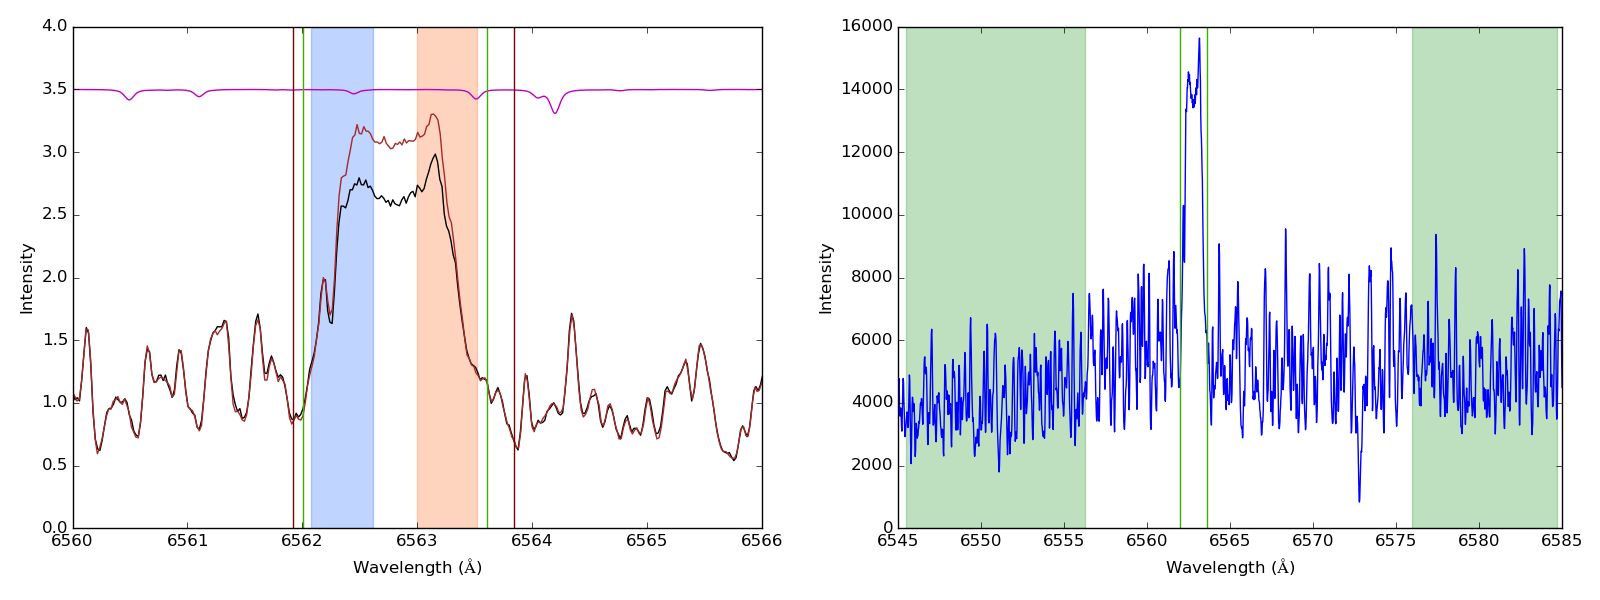
\includegraphics[scale=0.25]{Figures/harpsfirstha4.png} \\
\end{center}   
\caption{In the left panel the {\ha} region of example spectra of {\prox} taken from {\harps} on 27 May 2004 02:10:14
  UTC (black) and 15 March 2006 09:16:35 (brown) are depicted. In the right panel a larger region is selected, just for
  the earlier spectrum in the left panel, however without normalisation. The region delineated with the dark red solid
  vertical lines shows the region used for calculation of the {\ha} equivalent width in this \paperorthesis. The regions
  shaded in red and blue respectively show the regions used for calculation of the sizes of the two \horn s. The solid
  vertical green lines and green shaded areas in the right panel show the regions for calculation of the {\ha} index in
  other papers. The shaded dark green region in the right panel from 6572.468{\AA} to 6573.288{\AA} show the prominent
  TiO I transition line referred to in Section \ref{section:alternativelines}.
}
 \protect\label{fig:harpsfirstha}
\end{figure}

in Table \ref{table:ewtabfirst} are listed the Equivalent Widths, {\ha} Index and Peak Ratios from the {\uves} and
{\harps} data for {\prox}. Histograms of the Equivalent Widths are shown in Fig. \ref{fig:proxhists}. Note
that all the Equivalent Widths from the {\uves} data are displayed, but the seven very highest from the {\harps} data are
omitted, which have Equivalent Widths of over 6, which are listed in Table \ref{table:excessews}.

\begin{table}[!htbp]
\centering
\scalebox{0.75}{
\begin{tabular}{|l|l|l|r|c|c|c|}
\hline
Spectra & From & To & No. & EW & {\ha} Ind & PR \\\hline
\multirow{4}{*}{\uves} & 10/03/2009 & (same) & 215 & 1.759 $ \pm $ 0.301 & 1.759 $ \pm $ 0.301 & 0.850 $ \pm $ 0.021 \\
& 12/03/2009 & (same) & *166 & 1.324 $ \pm $ 0.258 & 1.324 $ \pm $ 0.258 & 0.907 $ \pm $ 0.014 \\
& 14/03/2009 & (same) & 179 & 1.492 $ \pm $ 0.560 & 1.492 $ \pm $ 0.560 & 0.921 $ \pm $ 0.025 \\\cline{2-7}
& \multicolumn{2}{|c|}{ALL} & 560 & 1.570 $ \pm $ 0.428 & 1.570 $ \pm $ 0.428 & 0.899 $ \pm $ 0.036 \\\hline
\multirow{7}{*}{\harps} & 27/05/2004 & 21/07/2004 & 6 & 2.711 $ \pm $ 7.105 & 0.248 $ \pm $ 0.416 & 1.013 $ \pm $ 0.024 \\
& 25/07/2005 & 22/03/2006 & 5 & 1.407 $ \pm $ 0.479 & 0.176 $ \pm $ 0.027 & 0.975 $ \pm $ 0.011 \\
& 14/03/2007 & 19/07/2007 & 5 & 2.012 $ \pm $ 0.542 & 0.210 $ \pm $ 0.031 & 0.999 $ \pm $ 0.010 \\
& 29/06/2008 & 06/04/2010 & 25 & 2.212 $ \pm $ 0.740 & 0.222 $ \pm $ 0.043 & 1.001 $ \pm $ 0.016 \\
& 19/02/2011 & 03/06/2011 & 12 & 2.290 $ \pm $ 4.518 & 0.225 $ \pm $ 0.271 & 0.990 $ \pm $ 0.025 \\
& 18/01/2013 & 10/01/2014 & 207 & 2.004 $ \pm $ 1.004 & 0.210 $ \pm $ 0.059 & 0.994 $ \pm $ 0.017 \\
& 19/01/2016 & 30/03/2016 & 56 & 2.882 $ \pm $ 2.974 & 0.262 $ \pm $ 0.175 & 1.006 $ \pm $ 0.017 \\\cline{2-7}
& \multicolumn{2}{|c|}{All (original set)} & 260 & 2.011 $ \pm $ 1.837 & 0.211 $ \pm $ 0.108 & 0.994 $ \pm $ 0.017 \\
& \multicolumn{2}{|c|}{All (full set)} & 316 & 2.115 $ \pm $ 2.136 & 0.217 $ \pm $ 0.126 & 0.997 $ \pm $ 0.018 \\\hline
\end{tabular}}
\caption{Results for calculation of median and standard deviation {\ha} equivalent widths (EW), {\ha} Index and peak ratio (PR) for {\uves} and
  \harps. In the {\uves} table all the spectra are used and the results shown by day and for all,
  *apart from an observation clearly consisting of noise only timed at
  12/03/09 02:31:11 UTC. In the {\harps} table the observations are separated where they are 300 or more days apart. In
  the summary lines ``original set'' refers to the observations up to 10/01/2014 and the ``full set'' also includes data
  from 19/01/2016 to 30/03/2016.}
\protect\label{table:ewtabfirst}
\end{table}

\begin{figure}[!htbp]
\begin{center}
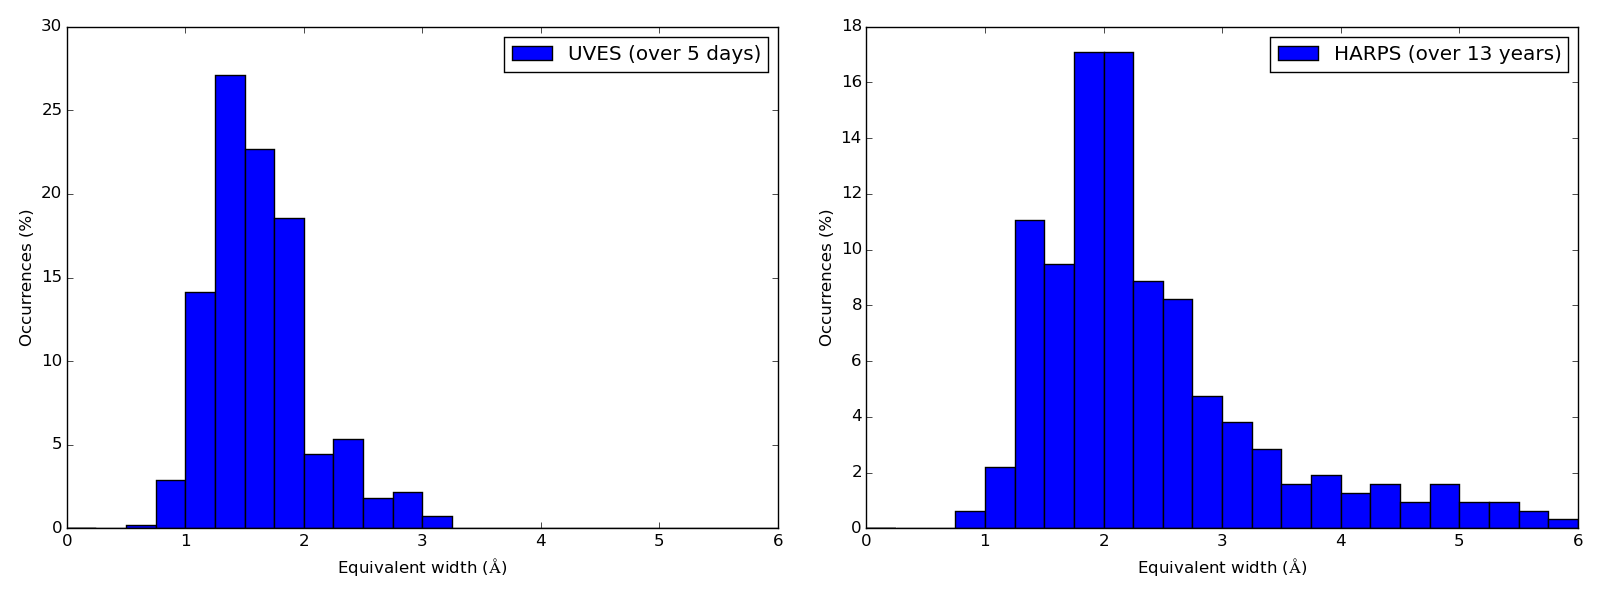
\includegraphics[scale=0.25]{Figures/proxhists.png} \\
\end{center}
\caption{Histogram of equivalent widths for {\uves} on the left and {\harps} on the right with the same X axis
  scale. All the {\uves} spectra results are shown apart from those for one which appeared to be just noise (12
  March 2009 UTC 02:31:11). {\harps} spectra are omitted for four outlying cases which appeared to be dominated by
  flares.}
 \protect\label{fig:proxhists}
\end{figure}
% Done with 25 bins scale 0:6

This {\paperorthesis} investigates calculations of periodicity from skewness, kurtosis and residual {\ha} lines. The residuals were
created by division of each spectrum by the spectrum with the lowest measured Equivalent Width and also the mean of the
5 spectra with the lowest equivalent widths. (See Section \ref{section:harpsper} below). The same two spectra which are
displayed in the left panel of Fig. \ref{fig:harpsfirstha} are re-displayed after this treatment in
Fig. \ref{fig:harpsfirsthad5}.

\begin{figure}[!htbp]
\begin{center}
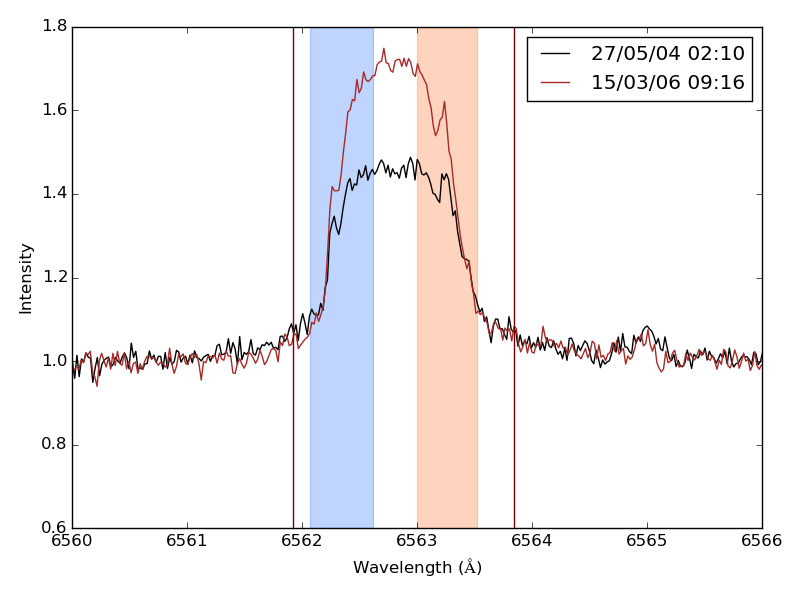
\includegraphics[scale=0.25]{Figures/harpsfirsthad5.png} \\
\end{center}   
\caption{This figure shows the residuals of the same two spectra as previously shown in the left panel of
 Fig. \ref{fig:harpsfirstha} after division by the mean of the first five spectra with minimum equivalent width
timed at 16 March 2006 UTC 06:37:59, 14 March 2007 UTC 07:28:29, 5 April 2011 UTC 03:26:33, 8 April 2011 UTC 06:28:17
and 22 April 2011 UTC 05:07:46.}
\protect\label{fig:harpsfirsthad5}
\end{figure}

\Notnow{
\begin{table}[!htbp]
\centering
\scalebox{0.75}{
\begin{tabular}{|l|l|r|c|c|}
\hline
From & To & No. & EW & PR \\\hline
%\multirow{11}{*}{Div by 1} & 27/05/04 & 21/07/04 & 6 & 1.167 $ \pm $ 4.633 & 1.062 $ \pm $ 0.032 \\\hline
%& 27/05/04 & 21/07/04 & $\dagger$5 & 0.699 $ \pm $ 0.952 & 1.043 $ \pm $ 0.023 \\\cline{2-6}
%& 25/07/05 & 22/03/06 & 5 & 0.346 $ \pm $ 0.290 & 1.016 $ \pm $ 0.014 \\\cline{2-6}
%& 14/03/07 & 19/07/07 & 5 & 0.732 $ \pm $ 0.338 & 1.039 $ \pm $ 0.011 \\\cline{2-6}
%& 29/06/08 & 06/04/10 & 25 & 0.828 $ \pm $ 0.458 & 1.046 $ \pm $ 0.015 \\\cline{2-6}
%& 19/02/11 & 03/06/11 & 12 & 0.877 $ \pm $ 3.005 & 1.037 $ \pm $ 0.027 \\\cline{2-6}
%& 19/02/11 & 03/06/11 & $\dagger$11 & 0.702 $ \pm $ 0.601 & 1.036 $ \pm $ 0.024 \\\cline{2-6}
%& 18/01/13 & 10/01/14 & 207 & 0.702 $ \pm $ 0.643 & 1.040 $ \pm $ 0.018 \\\cline{2-6}
%& 18/01/13 & 10/01/14 & $\dagger$205 & 0.701 $ \pm $ 0.580 & 1.039 $ \pm $ 0.018 \\\cline{2-6}
%& \multicolumn{2}{|c|}{ALL} & 260 & 0.704 $ \pm $ 1.199 & 1.040 $ \pm $ 0.019 \\\cline{2-6}
%& \multicolumn{2}{|c|}{ALL} & $\dagger$256 & 0.702 $ \pm $ 0.581 & 1.039 $ \pm $ 0.018 \\\hline
27/05/04 & 21/07/04 & 6 & 1.020 $ \pm $ 4.401 & 1.051 $ \pm $ 0.032 \\\hline
27/05/04 & 21/07/04 & $\dagger$5 & 0.577 $ \pm $ 0.903 & 1.035 $ \pm $ 0.022 \\\hline
25/07/05 & 22/03/06 & 5 & 0.243 $ \pm $ 0.273 & 1.004 $ \pm $ 0.015 \\\hline
14/03/07 & 19/07/07 & 5 & 0.609 $ \pm $ 0.320 & 1.026 $ \pm $ 0.011 \\\hline
29/06/08 & 06/04/10 & 25 & 0.698 $ \pm $ 0.433 & 1.034 $ \pm $ 0.014 \\\hline
19/02/11 & 03/06/11 & 12 & 0.744 $ \pm $ 2.862 & 1.030 $ \pm $ 0.025 \\\hline
19/02/11 & 03/06/11 & $\dagger$11 & 0.578 $ \pm $ 0.568 & 1.028 $ \pm $ 0.022 \\\hline
18/01/13 & 10/01/14 & 207 & 0.578 $ \pm $ 0.610 & 1.028 $ \pm $ 0.017 \\\hline
18/01/13 & 10/01/14 & $\dagger$205 & 0.577 $ \pm $ 0.550 & 1.028 $ \pm $ 0.017 \\\hline
\multicolumn{2}{|c|}{ALL} & 260 & 0.579 $ \pm $ 1.139 & 1.028 $ \pm $ 0.018 \\\hline
\multicolumn{2}{|c|}{ALL} & $\dagger$256 & 0.578 $ \pm $ 0.550 & 1.028 $ \pm $ 0.017 \\\hline
\end{tabular}}
\caption{This table re-displays the {\harps} spectra as previously shown in Table \ref{table:ewtabfirst} after
  calculating the residual spectra from dividing by the mean values of the 5 spectra with the lowest equivalent
  widths. As before, the rows marked {$\dagger$} show where equivalent   widths of greater  than 2 standard deviations
  from the median are removed and the median and standard deviations recalculated.}
\protect\label{table:divcompar}
\end{table}}

\section{Alternative lines to {\ha}}
\protect\label{section:alternativelines}

Although the {\ha} emission line is by far the strongest line on the {\prox} spectra, for comparison this study includes
some analysis of alternative lines and also with combining lines as suggested in \citet{hall99}, however the Equivalent
Widths, with appropriate scaling as the {\ha} line is so much greater in size than the others, are combined rather than
the fluxes as in that paper.

A prominent absorption line consistent across the spectra was identified to be a TiO transition at 6572.468{\AA} to
6573.288{\AA}, highlighted as the dark green shading in the right panel of Fig. \ref{fig:harpsfirstha}. This is enlarged
in Fig. \ref{fig:tispec}. The Equivalent Widths of this line and also the Peak Ratios from the {\harps} data in the same
manner as for Table \ref{table:ewtabfirst} and the results are shown in Table \ref{table:titable}.

\begin{figure}[!htbp]
\begin{center}
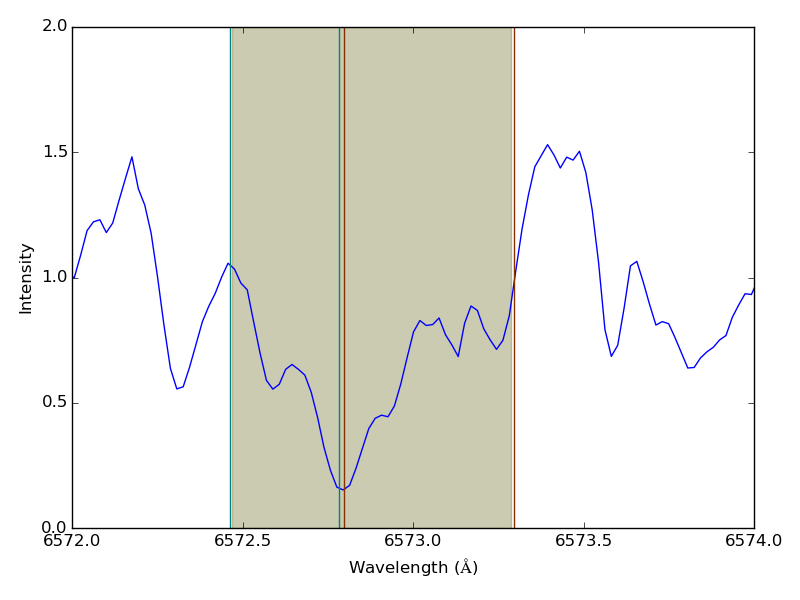
\includegraphics[scale=0.25]{Figures/tispec.png} \\
\end{center}   
\caption{This shows the section of the first spectrum in the {\harps} data (at 27 May 2004 UTC 02:10:14) used for
  calculating Equivalent Widths and also Peak Ratios from the TiO absorption line from 6572.468{\AA} to
  6573.288{\AA}. The blue vertical lines at 6572.463{\AA} and 6572.784{\AA} and the red lines at 6572.797{\AA} and
  6573.295{\AA} delineate the regions used for calculation of Peak Ratios.}
\protect\label{fig:tispec}
\end{figure}

\begin{table}[!htbp]
\centering
\scalebox{0.75}{
\begin{tabular}{|l|l|r|c|c|c|}
\hline
From & To & No. & EW  & Index & PR \\\hline
27/05/2004 & 21/07/2004 & 6 & 0.309 $ \pm $ 0.019 & 0.032 $ \pm $ 0.002 & 1.039 $ \pm $ 0.027 \\
25/07/2005 & 22/03/2006 & 5 & 0.314 $ \pm $ 0.004 & 0.032 & 1.017 $ \pm $ 0.012 \\
14/03/2007 & 19/07/2007 & 5 & 0.310 $ \pm $ 0.006 & 0.032 $ \pm $ 0.001 & 1.030 $ \pm $ 0.036 \\
29/06/2008 & 06/04/2010 & 25 & 0.315 $ \pm $ 0.007 & 0.031 $ \pm $ 0.001 & 1.020 $ \pm $ 0.035 \\
19/02/2011 & 03/06/2011 & 12 & 0.312 $ \pm $ 0.008 & 0.032 $ \pm $ 0.001 & 1.036 $ \pm $ 0.024 \\
18/01/2013 & 10/01/2014 & 207 & 0.310 $ \pm $ 0.006 & 0.032 $ \pm $ 0.001 & 1.047 $ \pm $ 0.027 \\
19/01/2016 & 30/03/2016 & 56 & 0.319 $ \pm $ 0.015 & 0.031 $ \pm $ 0.001 & 1.005 $ \pm $ 0.028 \\
\multicolumn{2}{|c|}{ALL} & 316 & 0.312 $ \pm $ 0.010 & 0.032 $ \pm $ 0.001 & 1.036 $ \pm $ 0.033 \\\hline
\end{tabular}}
\caption{Results for calculation of median and standard deviation of the equivalent widths of the TiO transition at 6572.468{\AA} to
6573.288{\AA} from \harps. The observations are separated where they are 300 or more days apart.}
\protect\label{table:titable}
\end{table}

As Table \ref{table:titable} shows, {\Firstp} also considered working with an ``index'' along the same lines as the {\ha}
Index, but considered the size and variations (0.032 $\pm$ 0.001) were too small to be useful.

\section{Flares on {\uves} data and X-ray values}
\protect\label{section:uvesflares}

In \citet[fig. 1 to fig. 3]{fuhrmeister11} the measured flux for various wavelengths for each of the three observation
nights are presented. In Fig. \ref{fig:uvrxp1} are displayed the {\ha} equivalent width and the X-ray counts for these
nights together with the peak ratios. As the X-ray flux is so much greater on the third day, the third panel is
potentially misleading, so these are re-displayed all to the same scale below in the bottom panel.

\begin{figure}[!htbp]
\begin{center}
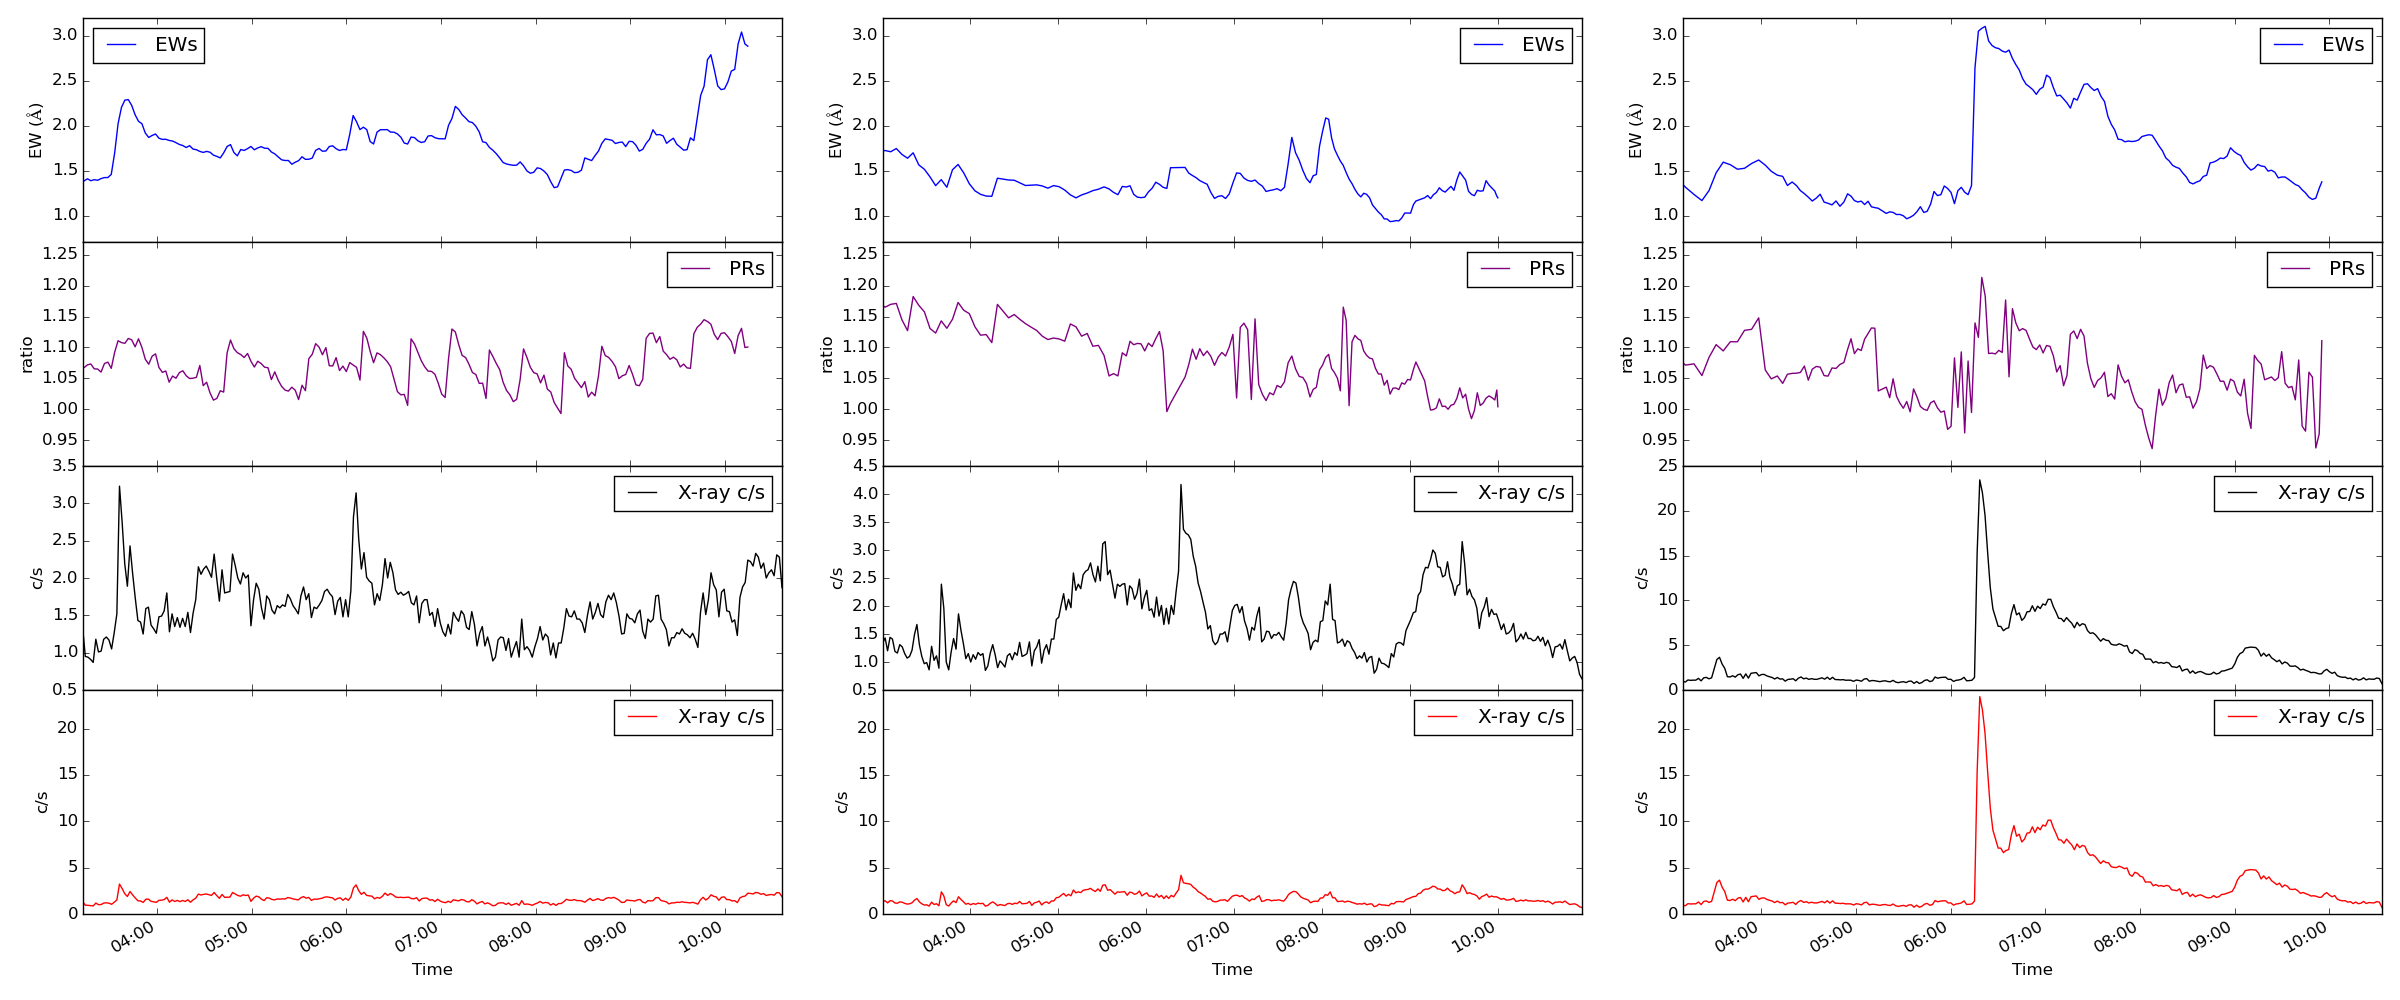
\includegraphics[scale=0.18]{Figures/uvrx-onepic.png} \\
\end{center}   
\caption{The horizontal panels from left to right are for each of the three days of the {\uves} data, 10, 12 and 14
  March 2009.  The Equivalent Width (top panel), Peak Ratio (second panel) and X-ray data (third and bottom panels) of the
  {\ha} flux as shown in \citet[Fig. 1 to Fig.3]{fuhrmeister11}. The top two panels are on the same scale
  throughout. The X-rays displayed are-displayed to the same scale on the fourth panel of each image.}
 \protect\label{fig:uvrxp1}
\end{figure}

In Fig. \ref{fig:uvrxp1} {\Firstp} noticed that the Peak Ratios for the first day (10 March 2009) seemed to have periodic nature for a portion of
the plot, as did a much smaller portion of the plot for the third day (14 March 2009). The portion on the first day had
a strong period of approximately half an hour and the third day a much weaker period of about 20 minutes.  However there
were no other periods found in the other day of a similar strength or value, either for Peak Ratios or Equivalent
Widths. However {\Firstp} noted that in \citet[Section 4.1]{barnes14} there is speculation of instrumentation error on
the first and third days applied to this data. By cross-correlation using the 6565-6585{\AA} region, {\Firstp} shifted
the spectra to compensate for apparent radial velocity variations. This enables {\Firstobj} to reduce the periodic
signal in the first day's plot and almost completely in the third day's plot.

%As these periods were not directly relevant to this project, focusing on the rotation period of
%\prox, {\Firstp} decided not to investigate this particular possible behaviour further until appropriate data is
%available.

The {\uves} data showed a large flare during the third of the observation periods starting at approximately 06:15 on
14th March 2009. Both the equivalent width and X-ray counts rapidly reached a peak, with the equivalent width peaking
approximately a minute before the X-ray count peaked. The equivalent width reached a similar level at the end of the
first observation period to that which it reached during the flare in the third, albeit much more slowly, but with only
very slight evidence of a corresponding increase in the X-ray count. However there was an increase in the {\uves}
optical''blue'' flux on the first day, as shown in \citet[fig. 1]{fuhrmeister11} corresponding to the higher Equivalent
Widths suggestive of an alternative temperature.

There is no corresponding X-ray data available for the {\harps} data, but as the {\uves} data suggests that {\ha}
Equivalent Width increases with flares, {\Firstp} selected the higher values of Equivalent Width in the {\harps} data as
indicative of flares. After some experimentation with investigation of periodicity, the effects of possible flares seemed to be
minimised if the proportion of data with the lower 90\% of Equivalent Widths were selected. In both {\uves} and {\harps}
this was approximately one standard deviation from the median, 2.0 in the case of {\uves} and 3.8 in the case of
{\harps}.

The {\harps} data contains four spectra with large values of Equivalent Width at 16 July 2004 UTC 01:52:40, 27 March
2011 UTC 05:20:09, 05 May 2013 UTC 03:31:16 and 5 May 2013 UTC 03:41:47 with values of 21.69, 18.12, 6.76 and 6.19
respectively.  {\FirstP} also noted that these spectra had a noticeable He-6678 line associated with these which appears
at first analysis to disappear rapidly after the peaks, not appearing significantly on higher {\ha} Equivalent Width
values outside those four spectra, suggesting that those four might be major flares.

\begin{table}[!htbp]
\centering
\scalebox{0.75}{
\begin{tabular}{|l|r|r|}
\hline
Epoch & EW & He-6678 \\\hline
18/03/2016 UTC 08:59:02 & 23.991 & 0.853 \\
16/07/2004 UTC 01:52:40 & 21.693 & 0.312 \\
27/03/2011 UTC 05:20:09 & 18.123 & 0.591 \\
31/01/2016 UTC 08:51:35 & 7.298 & 0.099 \\
26/02/2016 UTC 09:07:05 & 6.898 & 0.110 \\
05/05/2013 UTC 03:31:16 & 6.756 & 0.276 \\
05/05/2013 UTC 03:41:47 & 6.192 & 0.177 \\\hline
\end{tabular}}
\caption{The seven spectra with Equivalent Widths over 6, in descending order.}
\protect\label{table:excessews}
\end{table}

Regarding these lines find that the He-6678
line, highlighted in \citet[fig. 8]{fuhrmeister08} in relation to flares on CN Leonis, is visible in the spectra with
{\ha} Equivalent values of above 5.5, including the seven lines omitted. A comparison is shown in Fig. \ref{fig:dualews}.

\begin{figure}[!htbp]
\begin{center}
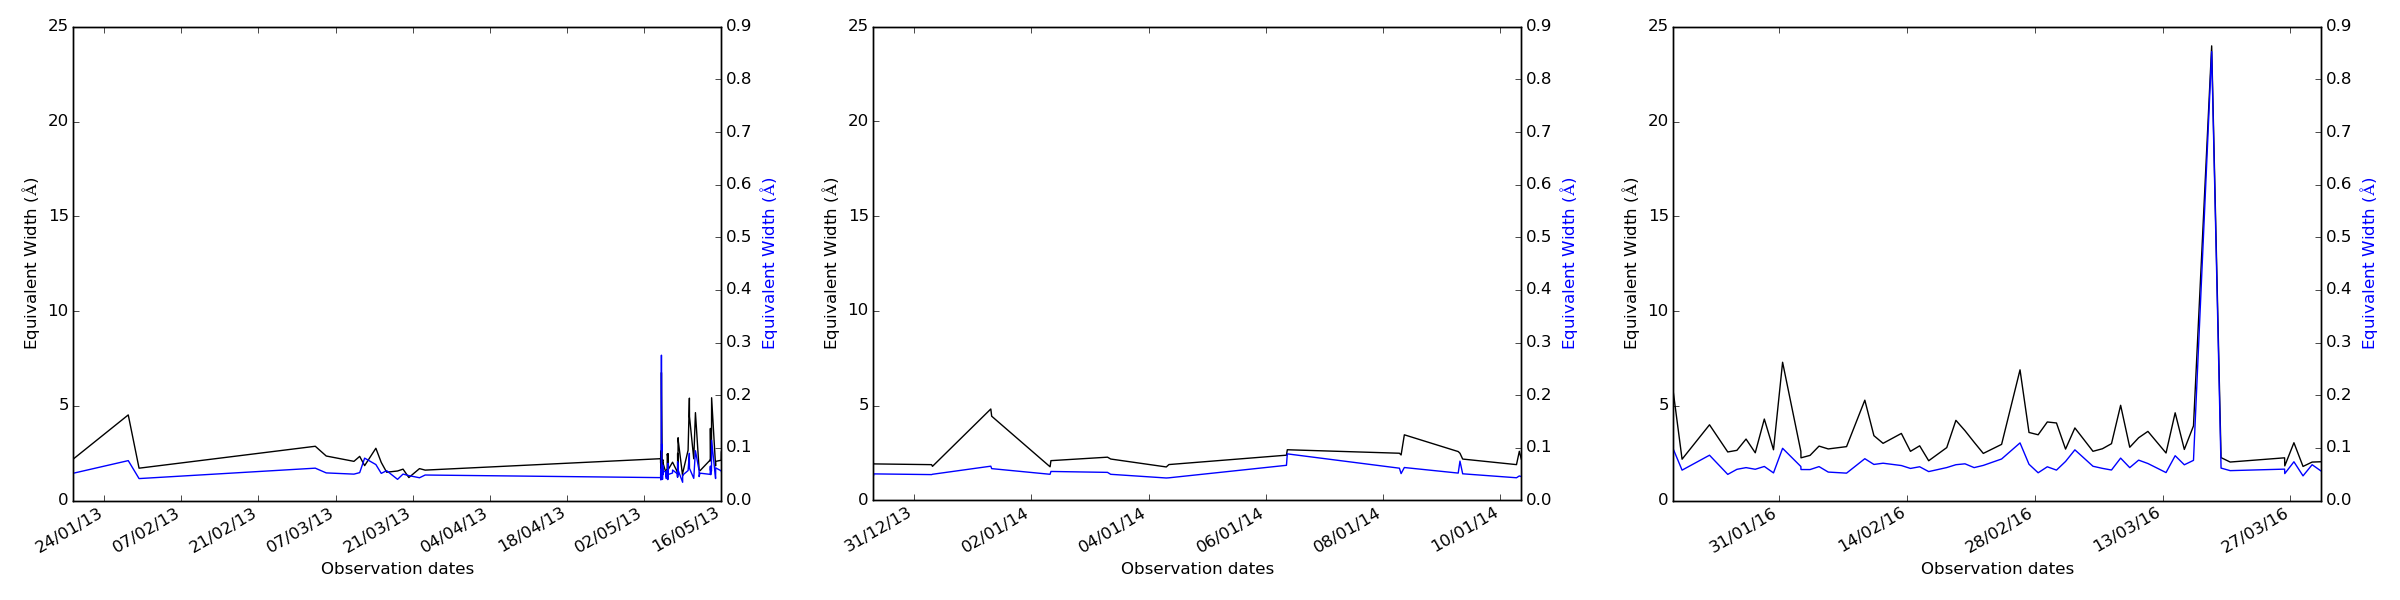
\includegraphics[scale=0.18]{Figures/dualcomb.png} \\
\end{center}   
\caption{The plots show the {\ha} Equivalent Width in black and the He-6678 Equivalent Widths in blue for the {\harps}
  observations in the years 2013, 2014 and 2015.}
 \protect\label{fig:dualews}
\end{figure}

\section{Recovery of periods from {\harps} data}
\protect\label{section:harpsper}

Attempts to derive periodograms from the results of the the various measures listed in Section \ref{section:linemeas}
met with much less success than the photometric results from {\asas} and {\hst}, in that, as discussed in Appendix
\ref{chapter:lsroutines} and listed in detail in Appendix \ref{chapter:pgramdetail}, all the various Lomb-Scargle
routines gave very different results for almost every line measure or combination of measures. A full list of results is
shown in Appendix \ref{chapter:pgramdetail}, showing the relative performance of the different routines and different
line measurements. The {\numrecs} routine usually failed to find periods close to the 82.6 day period identified in the
photometric results or on the occasions when it found it, gave a FAP at or very close to 1.0.

To examine the performance as well as possible, all the three Python routines described in Appendix
\ref{chapter:lsroutines} were tried with every set of data and the results compared. None of the routines gave any
meaningful results for below 40 days, with a plethora of strong peaks down to fractions of a day, or above 120 to 130
days, so all the periodograms were generated with periods between 40 and 130 days, in steps of 0.01 days (14 minutes, 20
seconds). This encompassed the 41.3 days of \citet{benedict93}, although this looks very likely to be a half-period
alias, through to and including the 116.6 days of \citet[Table 3]{suarezmascareno15} and encompassing the minimum period
of 50 days given by \citet{kurster99} and the 82 days of \citealt{benedict92,benedict98,kiraga07}. The erratic behaviour
of the periodograms below about 40 days made it impractical to extend the search down to include the 31.5 days of
\citet{guinan96}, but in the light of the photometric results and the unanimity of other reports as to the period being
longer than this, it was deemed not to matter.

Many of the periodograms showed several strong peaks all over the range searched, typically with up to five outstanding
peaks in the range searched, so for this {\paperorthesis} note was taken of the periods of the strongest peaks and of
the five strongest peaks in the analyses of the periodograms.

In Fig. \ref{fig:harpspgrams1} is shown how the different routines give different results with identical data; the upper
panel showing the results from the {\astroml} routine and the lower panel showing the results from {\gatspy}. In
Fig. \ref{fig:harpspgrams2} is shown a result from Peak Ratio calculation giving a value of 82.2 days returned by
\gatspy.

\begin{figure}[!htbp]
\begin{center}
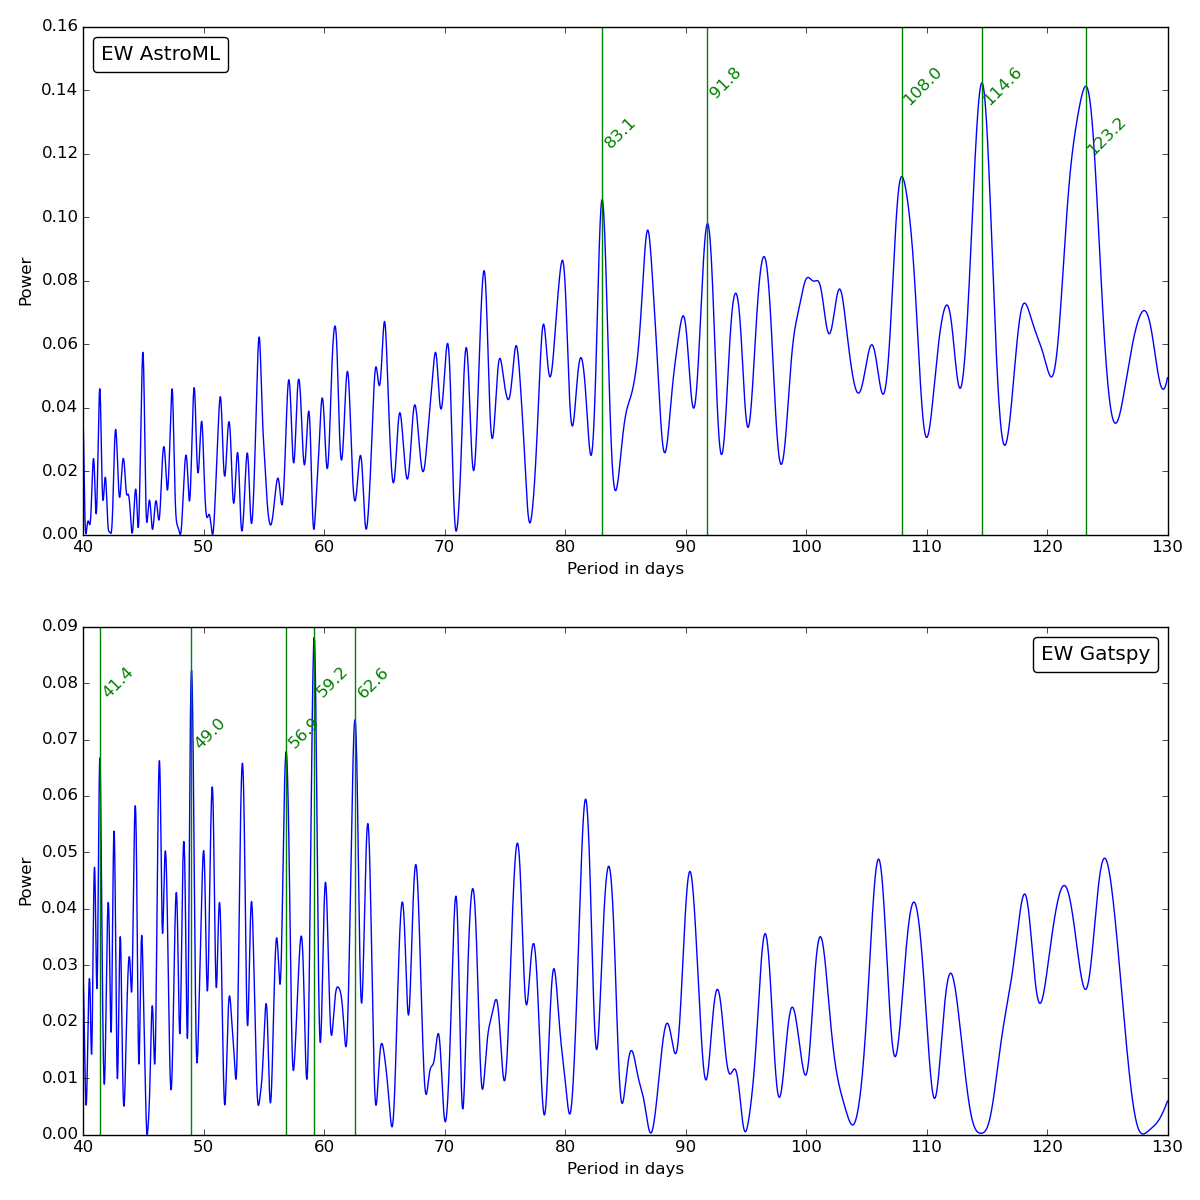
\includegraphics[scale=0.20]{Figures/summpgrams.png} \\
\end{center}   
\caption{This figure shows sample periodograms from the {\ha} peak of the {\harps} data, calculating from Equivalent
  Widths using {\astroml} for the upper panel and {\gatspy} for the lower panel. This corresponds to the second and
  third rows of Table \ref{table:fullewtaball}. The strongest 5 peaks are highlighted in both cases.}
\protect\label{fig:harpspgrams1}
\end{figure}

\begin{figure}[!htbp]
\begin{center}
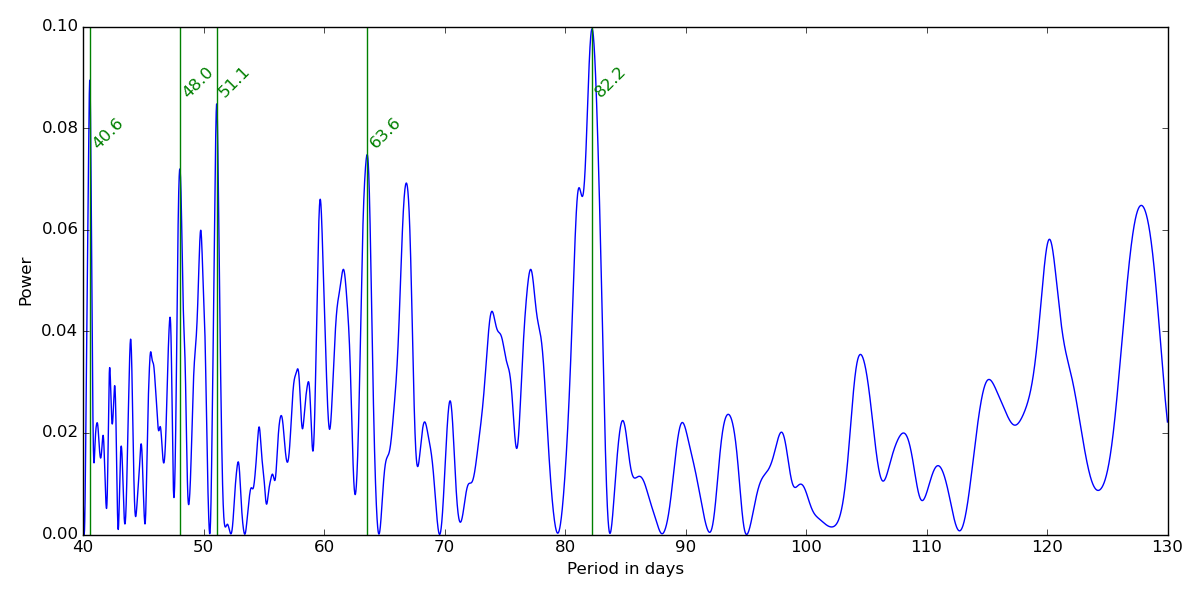
\includegraphics[scale=0.40]{Figures/harpsprbind1.png} \\
\end{center}   
\caption{This figure shows a sample periodogram from the Peak Ratio measure from the Full Set of the data from {\harps}
  binned to 1 day, processed by the {\gatspy} routine and displayed with the five highest peaks highlighted and showing
  the values. This corresponds to the ninth row Table \ref{table:fullprtaball}.}
\protect\label{fig:harpspgrams2}
\end{figure}

Some efforts were made to remove data contaminated from flares, either by clipping spectra with various upper bounds of
Equivalent Width, by binning data or both. Following the lead from {\uves} in Section \ref{section:uvesflares}, spectra
were clipped where the Equivalent Width exceeded one standard deviation from the median. This was 3.8 for the Original
Set or 4.2 for the Full Set of data. However the latter, which included some spectra with very large equivalent widths
taken in 2016, did not yield any particular benefit, so with the full set of data, clipping to a maximum Equivalent
Width of 3.8 in line with the Original Set was tried. Binning to 1 day was attempted as was binning to 0.5 days. In
terms of effectiveness 

The results from the {\ha} Index were almost identical to those from the Equivalent Width measure, so in the majority of
the tables the latter is focused upon, together with Peak Ratios, Skewness and Kurtosis. The full results for these are
found in Appendix \ref{chapter:pgramdetail} and tables \ref{table:origewtaball}, \ref{table:fullewtaball},
\ref{table:origprtaball}, \ref{table:fullprtaball}, \ref{table:origskewtaball}, \ref{table:fullskewtaball},
\ref{table:origkurttaball} and \ref{table:fullkurttaball}. In Table \ref{table:perftable} below these tables in Appendix
\ref{chapter:pgramdetail} are summarised by summarising the occurrences of 82.6 days in the first five peaks within 0.5\%
and 2\% and either 82.6 or the half-period of 41.3 days to the same percentages.

\begin{table}[!htbp]
\centering
\scalebox{0.75}{
\begin{tabular}{|l|l|r|r|r|r|}
\hline
\textbf{Measure}&\textbf{Data set}&\multicolumn{2}{|c|}{\textbf{82.6 days}}&\multicolumn{2}{|c|}{\textbf{82.6 or 41.3 days}}\\\hline
&&\textbf{Up to 0.5\%}&\textbf{Up to 2\%}&\textbf{Up to 0.5\%}&\textbf{Up to 2\%}\\\hline
\multirow{2}{*}{Peak Ratio}&Original&38 & 62 & 48 & 76\\
&Full&47 & 53 & 47 & 60\\\hline
\multirow{2}{*}{Equivalent Width}&Original& 5 & 5 & 43 & 43\\
&Full&3 & 57 & 30 & 83\\\hline
\multirow{2}{*}{Skewness}&Original&0 & 24 & 0 & 24\\
&Full&0 & 40 & 10 & 50\\\hline
\multirow{2}{*}{Kurtosis}&Original&0 & 29 & 0 & 29\\
&Full&17 & 27 & 17 & 27\\\hline
\end{tabular}}
\caption{This table summarises the approximate recovery performance in terms of finding the expected period of 82.6 and
  this or the half-period of 41.3 within the first five peaks and within a given percentage considering all line measurement methods employed with the
  original and full data. All clipping and binning of the data is included in the summary for each method. The full data
  is listed in Appendix \ref{chapter:pgramdetail}.}
\protect\label{table:perftable}
\end{table}

\section{Comparison of {\asas} and {\harps} for period recovery}
\protect\label{section:asasfap}

It seemed appropriate to look in more detail at the {\asas} data which offers similar sampling to that from the {\harps}
data discussed in Section \ref{section:harpsper} above. Of particular importance is the False Alarm Probability of
periods recovered from the spectroscopic data as well as estimating the uncertainty level of all of the calculated
periods, particularly those in the Photometric data. None of the three Python routines directly return an FAP and the
the {\numrecs} routine always returns an FAP of 1 for the periods if the periods were found at all. Consequently a Monte
Carlo method was devised and implemented to study this and at the same time help estimate the uncertainty on the period
obtained from the {\asas} results.

The {\asas} data has many more observations than the spectroscopic data from {\harps}. The former has 970 and the latter
has 316 (or 260 in the Original Set). If the {\asas} data is binned, then as noted in Section \ref{section:asas}, the
number of observations becomes 924 if binned to the most optimal 18 minutes or 624 if binned to 1 day, more akin to the
binning used in many of the periodicity calculations for the {\harps} data, and a more manageable ratio of numbers of
observations.

So, starting from the {\asas} data, binned to 1 day and assuming for the purpose that the 82.6 day period obtained from
the full set as described in Section \ref{section:asas} is correct, various percentage-sized subsets of the data were
randomly selected, recalculating the periods, noting whether a value close to the correct period was recovered as the
strongest peak, within the five strongest peaks, or not at all. If the period was recovered, the RMS error, assessed as
the difference from 82.6 days, was recorded. The sizes of the subsets were taken between 5\% and 95\% in steps of
5\%. For each percentage sized subset, the process was repeated 2,000 times. The results are illustrated in
Fig. \ref{fig:asasprop}.

In Fig. \ref{fig:asasprop} is shown four results. In all cases the X-axis displays the percentage sized subset of the
binned {\asas} data which was used. On the left Y-axis is shown the percentage of recovery (i.e. 100\% minus the FAP) of
the correct period. The blue line shows the percentage recovery of the correct period as the strongest peak with various
percentage sized subsets of the data and the green line shows the percentage recovery of the correct period as one of
the five strongest peaks, not necessarily as the strongest peak. If can be seen that former reaches 100\% recovery at
about 70\% and the latter at about 45\%.

On the right Y-axis is shown the RMS error in the period when it is correctly-recovered period. The purple line shows
the RMS error in the results corresponding to the case where the correct period is recovered as the strongest peak and
the red line the RMS error in the results corresponding to the case where the correct result is found in one of the top
five peaks. It is noticeable that this reaches less than 0.1 days in both cases, lending weight to the conclusion that
the uncertainty in the 82.6 peak found by {\asas} and {\hst} is of the order of 0.1 days at worst.

Finally, marked in as the dotted vertical black lines are the percentages where various numbers of observations with
various clippings and binnings of the {\harps} data would come. The actual numbers of observations range from 55, or
8.8\% of 624, to 316, or 50.6\% of 624. The intersections with the blue lines would indicate the level of FAP which
would be expected from the most powerful peak in the corresponding periodogram and that with the green lines would
indicate the level of FAP as one of the top five peaks. This can be considered alongside the summary in Table
\ref{table:perftable} but that is a condensation of the results in Appendix \ref{chapter:pgramdetail}, some of which
have a larger number of observations than others. It is clear that the best view of the performance from the
spectroscopic methods -- 53\% of the results for Peak Ratio, accepting periods within 2\% is poorer, both in terms of
rate of recovery and in error bar, than could be explained by restriction of the points alone - i.e. about 70\%.

\begin{figure}[!htbp]
\begin{center}
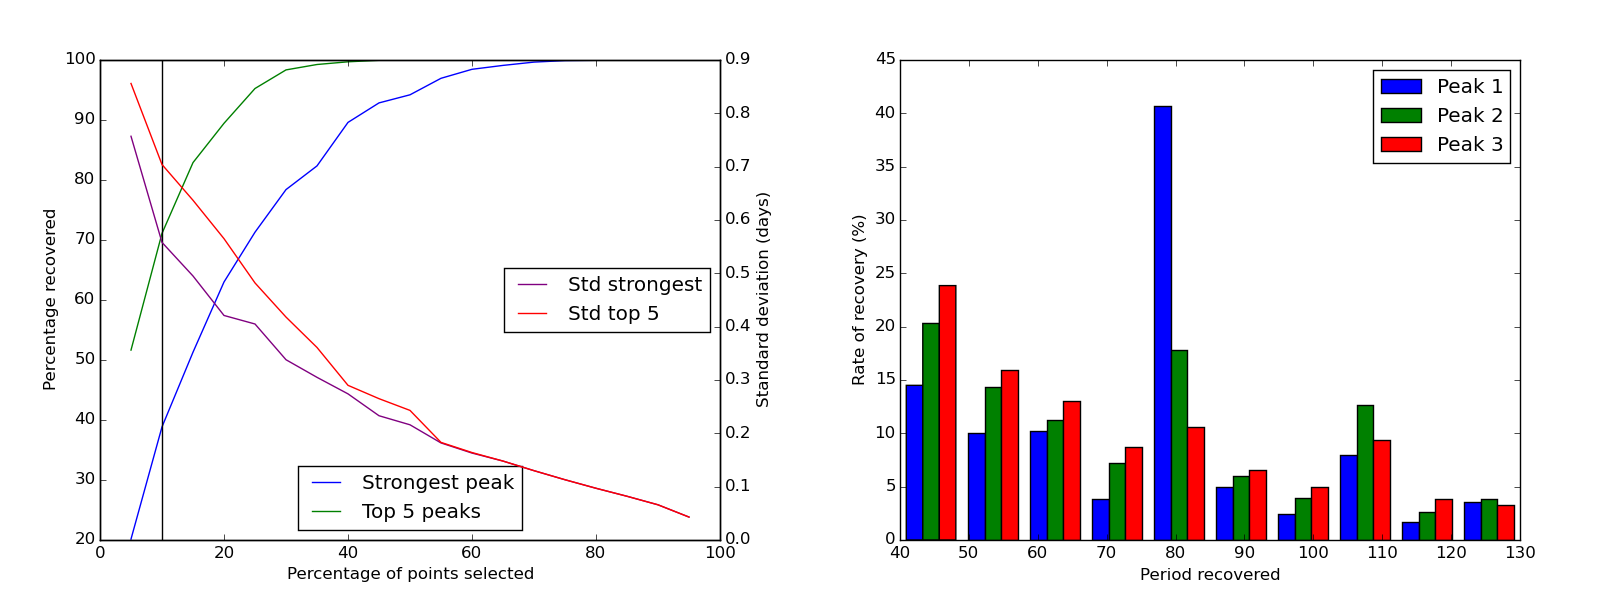
\includegraphics[scale=0.4]{Figures/prop.png} \\
\end{center}   
\caption{In this figure is illustrated the effects of randomly selecting a given proportion of the {\asas} data in terms
  of whether the same period of 82.6 days is recovered and the error in this result. The black vertical dotted lines
  mark in the proportions of data corresponding to the number of observations in the various clippings and binnings of
  the data listed in Table \ref{table:origewtaball} and Table \ref{table:fullewtaball}.}
\protect\label{fig:asasprop}
\end{figure}

\chapter{Modelling of {\prox} spectra}
\protect\label{chapter:modelling}
\lhead{Chapter \ref{chapter:modelling} \emph{Modelling of {\prox} spectra}}

In order to develop and refine the methods for evaluation of the periodicity of the sub-peaks in the {\prox} spectra, a
version of the ``Doppler Tomography of Stars'' (DoTS) modelling software \citep{CCamerondotsa} was used. Although DoTS
was written to recover surface imhomogeneities from time series spectra, here the forward modelling routines were used
to generate synthetic spectra, with some modifications. Specifically, \examrevision{a 3D model of the star, but with a 2D
  spherical model of the photosphere} was constructed, covered in a finite number of pixels. The intensity of each pixel
can vary from a photospheric value to a value appropriate for plage. In order to obtain the appropriate photospheric
intensity for each pixel at a given rotation phase of the stellar model,the 4-parameter limb darkening law introduced by
Claret from Phoenix model atmospheres \citep{claret00a} was used for an effective temperature of 3000K. The plage
intensities were calculated according to \citet[Section 4.1]{unruh99}, who identified the centre to limb variability
from plage regions relative to the photospheric (quiet) intensity for the Sun. Since no such observations exist for
other stars, the same \examrevision{centre-to-limb variation as for the solar plage was used relative to the photospheric
  centre-to-limb variation of \prox, selecting the limb-darkening law appropriate for the lower photosphere temperature
  and} with appropriate facular contrasts for {\ha} wavelengths (see \citet[figs 3 \& 4]{unruh99}).

Since it was desired to simulate the {\ha} line profile, a local intensity profile was assumed for the photosphere and
the plage. For inactive photospheres of \rdwarf s with similar spectral type to {\prox}, {\ha} is not visible (e.g. see
{\ha} profile in \citet[fig. 6]{barnes14} for GJ1061). Hence for the quiet photosphere, a flat continuum was assumed For
active stars, {\ha} possesses a characteristic emission profile with self-absorption, resulting in a double-peaked
profile. Since the {\vsini} is probably less than 0.1 km/s for \prox, the local line profile shape for {\ha} was based
on the observed {\prox} line profile since it is unlikely to show rotational broadening. This profile was tuned to
resemble the average {\ha} profile shown in the {\uves} data analysed in \citet{fuhrmeister11}, but symmetric about the
central wavelength. Specifically, a Gaussian profile was used to generate the emission peak and a second Gaussian with
narrow width to represent the central self-absorption as illustrated in Fig. \ref{fig:integregions}.  \examrevision{The
  profile was selected with the spread of wavelengths in resembling the {\ha} peak and with equivalent width so as to
  resemble the mean peak in the {\harps} data. The intensity could be fine-adjusted in the lookup-table parameters for
  the DoTS program so as to yield a variation in equivalent width comparable to that of the {\harps} observations
  ignoring those affected by flares with the selected plage distribution in use.}

\begin{figure}[!htbp]
\begin{center}
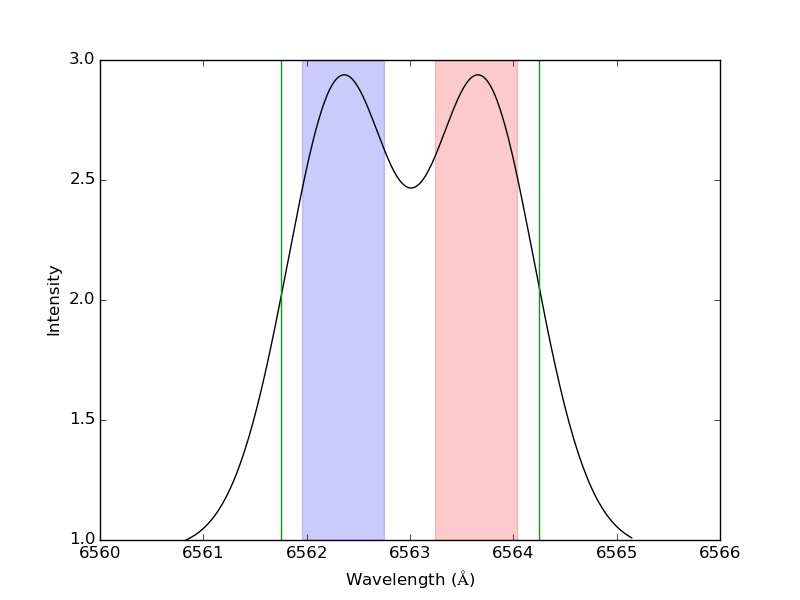
\includegraphics[scale=0.40]{Figures/integregions.png} \\
\end{center}
\caption{Example generated model spectrum of \prox, also illustrating the methods for computing the periodicity of
  spectra.  The centre of the \ha{} line is set at 6563{\AA} for convenience rather than 6562.8\AA{}.  The green lines
  (from 6561.75{\AA} to 6564.25\AA) show the limits used for calculation of the equivalent width. The blue and red
  shaded areas (6561.95{\AA} to 6562.75{\AA} and 6563.44{\AA} to 6564.24{\AA} respectively, each 0.8{\AA} wide) show the
  regions for calculation of the peak ratio.}
\protect\label{fig:integregions}
\end{figure}
% Done with 10 plage 80 period 75 deg first spectrum

With the two-temperature model, in subsequent simulations below, either photospheric intensity or a plage intensity is
assigned to each pixel. For a pixel containing plage, the synthetic {\ha} profile is scaled and for the photosphere with
no visible profile (as note above), the continuum level is used. The line profile is shifted appropriately for the
Doppler shift of each pixel in the model, \examrevision{however with the small Doppler shift due to the {\vsini} of less
  than 0.1 km/s on {\prox}, the main velocity variation observed is due to the asymmetry of the plage distribution}. The
model enables the user to place circular spots of specified radii anywhere on the star. For each viewing angle (or
equivalently observation phase), the appropriate intensity profiles of all visible pixels is calculated (according to
position on the line and centre-to-limb variation) and sum them to obtain the simulated line profile.

A model star with plage regions that rotate into and out of view can thus potentially exhibit variability in the line
shape since the pixels on different parts of the star possess different Doppler velocities. For stars such as \prox,
which probably possess a {\vsini} much less than the instrumental resolution, \examrevision{any velocity distortions in
  the the line profile due to spots rotating into and out of view will be insignificant or very small}. A plage region
that rotates into view may nevertheless have a significant effect on the the equivalent width of the simulated line
since the local intensity profile for {\ha} \examrevision{possesses a greater normalised peak intensity than} the
continuum. For stars with rotational velocity much greater than the instrument resolution, line asymmetries are likely
to be much more reliable.

\section{Plage distribution and results}
\protect\label{section:plagedists}

During the course of experimentation with models, a selection of plage distributions was tried, ranging from a single
large spot on one face to randomly-placed spots of random sizes. \examrevision{In all cases a 100\% filling factor for
  the plage was selected.} However it was found that the variation in equivalent widths from a low spot coverage was
bore no possible resemblance to that from observational data, in that the generated simulated spectra just exhibited two
extremes of equivalent widths and no intermediate values. On the other hand a coverage of more than about 30\% provided
very limited swings in the equivalent width compared those observed from {\harps} and {\uves}. After some
experimentation, a randomly distributed plage was settled upon which \examrevision{covered} up to 2.5\% of the surface,
towards the high end of the coverage of up to 2.7\% reported in \citet{guttenbrunner14} in relation to the Sun,
\examrevision{with the intensity parameters in the flux profile and the model adjusted to yield a variation in equivalent
  widths similar to the {\harps} observations}.

The models were all generated with the observation dates from the Original Set of {\harps}\footnote{This work was
  completed before the 2016 data was available. Also, as discussed in Section \ref{section:addflares}, it proved useful
  to study the Original Set of data as the 116.6 day period of \citet[Table 3]{suarezmascareno15} appeared in some
  cases, as illustrated in Fig. \ref{fig:rec116}.}, using possible rotation periods between 15 and 90 days in steps of 5
days and inclinations between 10{\degree} and 90{\degree} in steps of 5{\degree} to observe the various effects. Only a
limited selection, usually multiples of 10 days and 10{\degree} are shown in this {\paperorthesis} to conserve space.

In Fig. \ref{fig:extremew} some example spectra showing extremes of equivalent width and the median  are shown, and in
Fig. \ref{fig:extremewpics} the corresponding visible faces of the star with the plage spots marked in.

\begin{figure}[!htbp]
\begin{center}
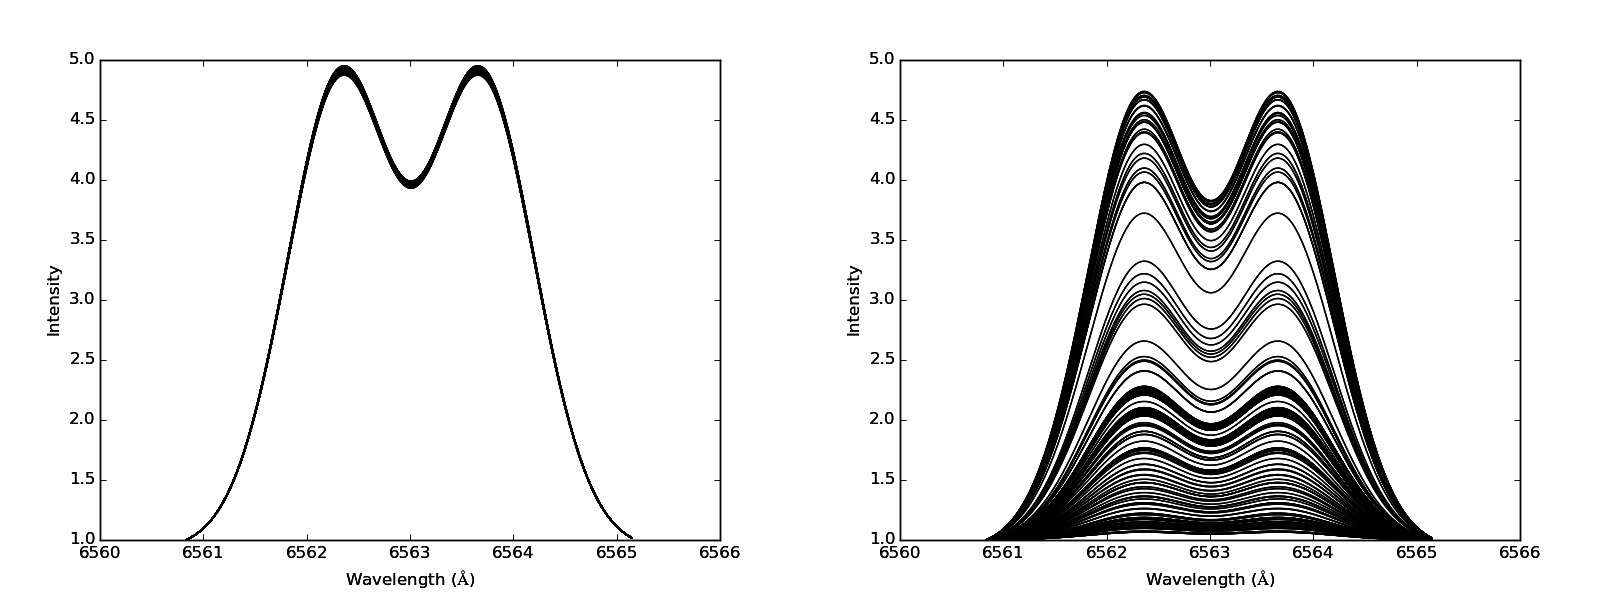
\includegraphics[scale=0.40]{Figures/extremes.png} \\
\end{center}
\caption{This displays simulated spectra showing the extremes and the median value of equivalent width (1.5, 3.0 and 2.3
  respectively) with a period of 80 days and an inclination of 80\degree. The epochs from the {\harps} data are used in
  the model and the selected generated spectra superimposed.}
\protect\label{fig:extremew}
\end{figure}

\begin{figure}[!htbp]
\begin{center}
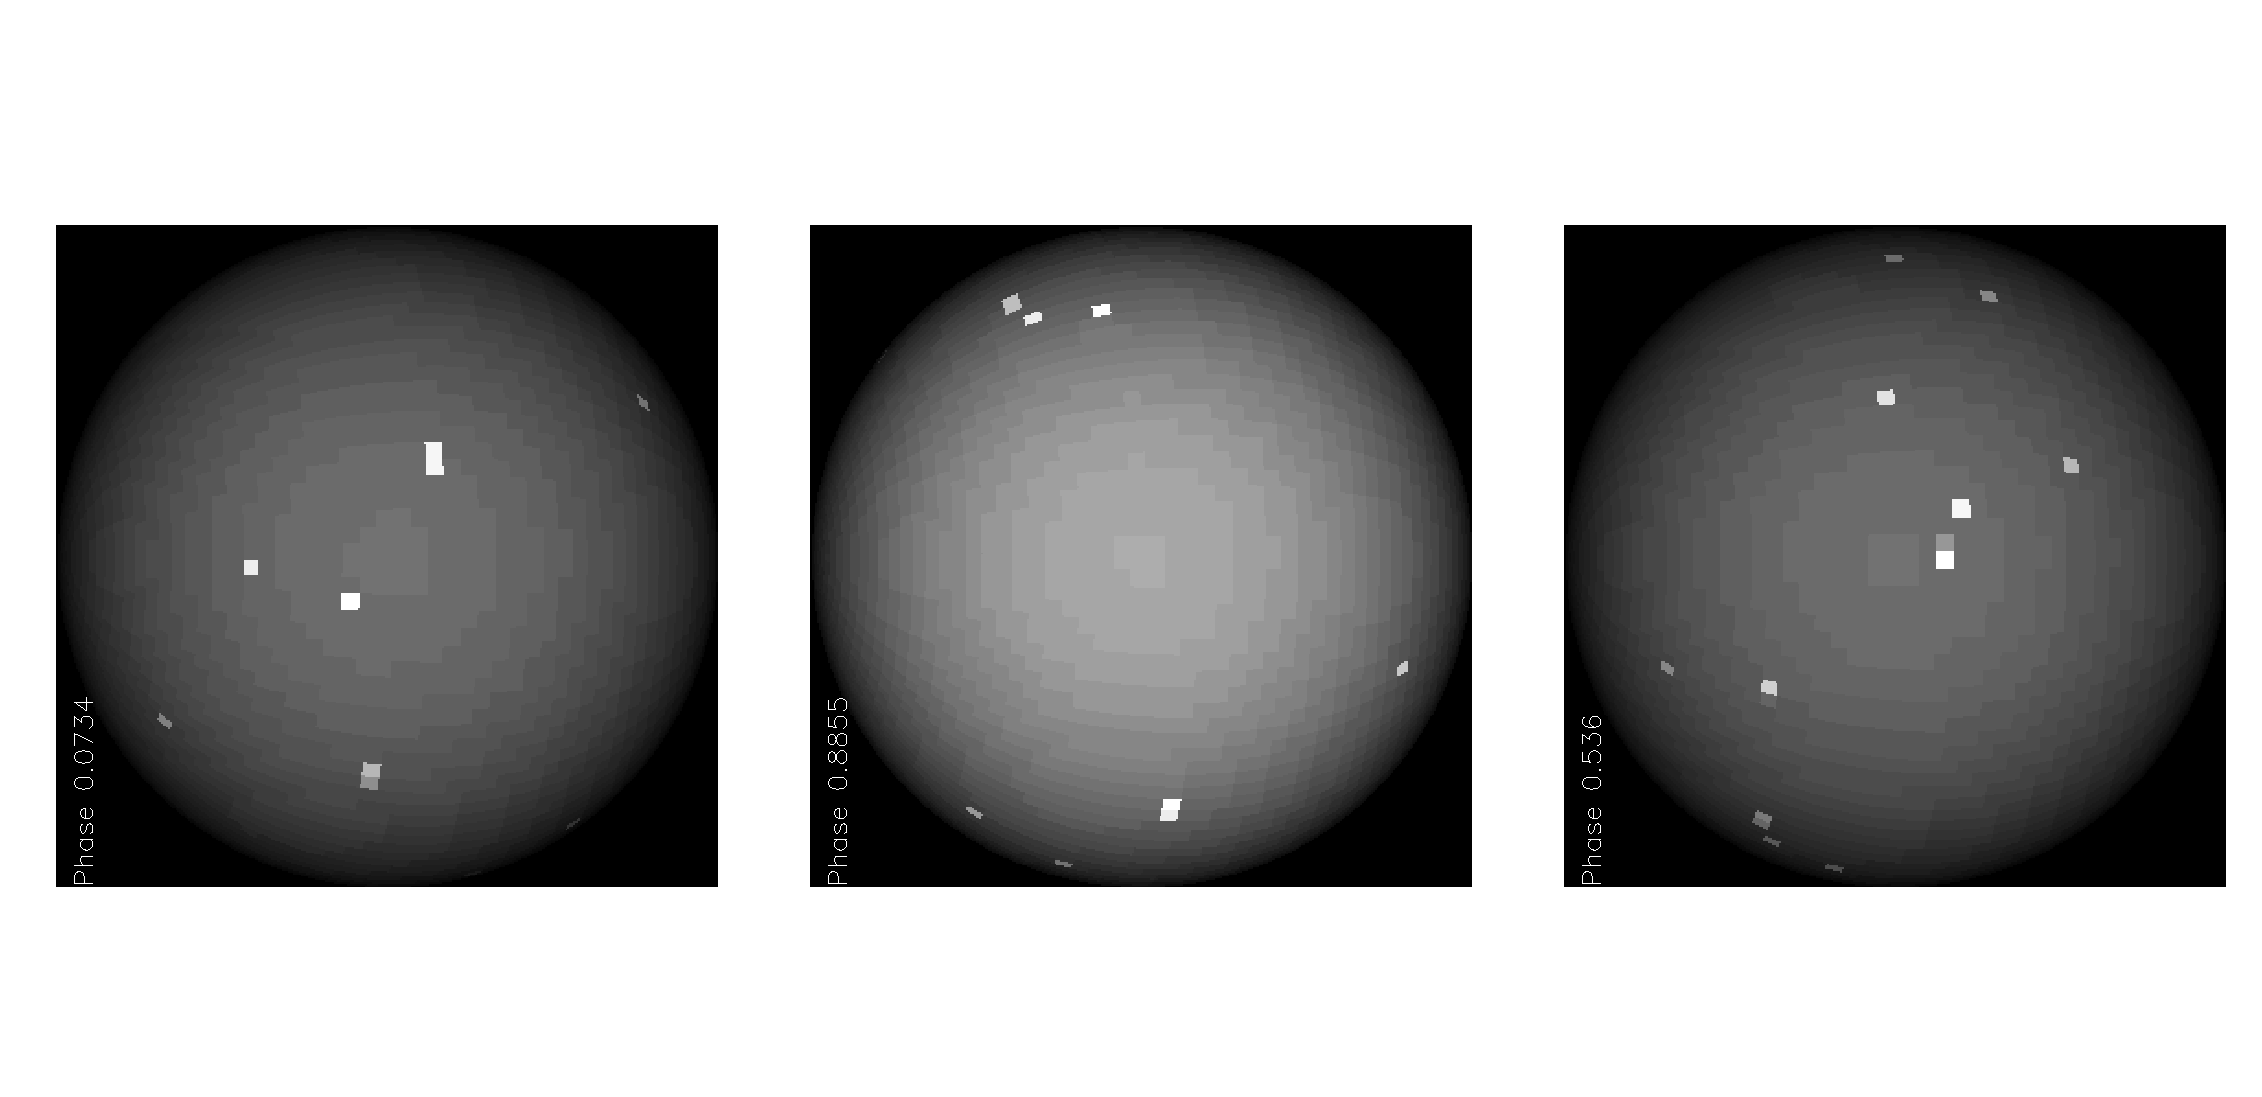
\includegraphics[scale=0.18]{Figures/extremeewpics.png} \\
\end{center}
\caption{This shows the visible face of the star as generated by DoTS corresponding to the spectra displayed in
  Fig. \ref{fig:extremew} in chronological order. Left to right, these give the spectra with the median, the lowest and
  the greatest equivalent widths.}
\protect\label{fig:extremewpics}
\end{figure}

In table \ref{table:modelcomp} are presented a selection of typical results showing means and standard deviations
for the equivalent width method (EW) with the two plage distributions for various periods and with 30{\degree},
60{\degree} and 90{\degree} inclinations and for 70, 80 and 90-day periods with 10{\degree} to 90{\degree} inclinations.
Note that the PR results are not displayed as variations were insufficient to be displayed in less than 6 figures, the
Doppler variations are just too insubstantial.

\begin{table}[!htbp]
\centering
\scalebox{0.75}{
\begin{tabular}{|l|c|l|l|l|}
\hline
Plage Dist & Period & \multicolumn{1}{|c|}{30\degree}&\multicolumn{1}{|c|}{60\degree}&\multicolumn{1}{|c|}{90\degree}\\\hline
\multirow{8}{*}{Random to 2.5\%} & 20 & 2.150 $ \pm $ 0.572 & 2.746 $ \pm $ 0.939 & 2.735 $ \pm $ 0.891  \\
& 30 &  2.725 $ \pm $ 0.495 & 3.870 $ \pm $ 0.895 &  4.004 $ \pm $ 0.942 \\
& 40 &  1.917 $ \pm $ 0.541 & 2.501 $ \pm $ 0.927 &  2.614 $ \pm $ 0.967 \\
& 50 &  1.604 $ \pm $ 0.483 & 1.996 $ \pm $ 0.805 &  2.018 $ \pm $ 0.876 \\
& 60 &  1.626 $ \pm $ 0.573 & 2.057 $ \pm $ 0.951 &  2.099 $ \pm $ 1.006 \\
& 70 &  1.967 $ \pm $ 0.445 & 2.334 $ \pm $ 0.803 &  2.340 $ \pm $ 0.821 \\
& 80 &  1.637 $ \pm $ 0.495 & 2.161 $ \pm $ 0.805 &  2.309 $ \pm $ 0.828 \\
& 90 &  2.475 $ \pm $ 0.548 & 3.365 $ \pm $ 0.894 &  3.410 $ \pm $ 0.901 \\\hline
\end{tabular}}

\vspace{5 mm}

\scalebox{0.75}{
\begin{tabular}{|l|c|l|l|l|}
\hline
Plage Dist & Incl\degree & \multicolumn{1}{|c|}{70 days}&\multicolumn{1}{|c|}{80 days}&\multicolumn{1}{|c|}{90 days}\\\hline
\multirow{9}{*}{Random to 2.5\%} & 10 & 1.693 $ \pm $ 0.140 & 1.484 $ \pm $ 0.182 & 1.816 $ \pm $ 0.196 \\
& 20 &  1.811 $ \pm $ 0.292 &  1.492 $ \pm $ 0.356 &  2.116 $ \pm $ 0.387 \\
& 30 &  1.967 $ \pm $ 0.445 &  1.637 $ \pm $ 0.495 &  2.475 $ \pm $ 0.548 \\
& 40 &  2.116 $ \pm $ 0.590 &  1.810 $ \pm $ 0.626 &  2.827 $ \pm $ 0.691 \\
& 50 &  2.237 $ \pm $ 0.711 &  1.994 $ \pm $ 0.732 &  3.139 $ \pm $ 0.815 \\
& 60 &  2.334 $ \pm $ 0.803 &  2.161 $ \pm $ 0.805 &  3.365 $ \pm $ 0.894 \\
& 70 &  2.392 $ \pm $ 0.860 &  2.277 $ \pm $ 0.848 &  3.477 $ \pm $ 0.930 \\
& 80 &  2.396 $ \pm $ 0.877 &  2.338 $ \pm $ 0.850 &  3.464 $ \pm $ 0.911 \\
& 90 &  2.340 $ \pm $ 0.821 &  2.309 $ \pm $ 0.828 &  3.410 $ \pm $ 0.901 \\\hline
\end{tabular}}
\caption{Simulated mean equivalent widths with associated standard deviations from simulations for the 2.7\%
  plage distributions and a set of rotation periods and inclinations. In the first table results are illustrated for
  various periods and for 30{\degree}, 60{\degree} and  90{\degree} inclinations. In the second table results are
  illustrated for various inclinations and 70, 80 and 90-day periods as these are close to the
  rotation period of \prox.}
\protect\label{table:modelcomp}
\end{table}

For each set of generated spectra for both plage distributions, rotation period (between 15 and 90 days in steps of 5
and inclination (between 10{\degree} and 90{\degree} in steps of 5\degree), a periodogram was obtained, viewing periods
between 10 days and 130 days in steps of 0.01 days, from the calculated equivalent widths and the RMS error over all
inclinations noted. In nearly all cases the error was rarely more than 0.02 days. It was rather a different matter for
the peak ratios however, in that the variations observed in the peak ratios were typically $2{\times}10^{-5}$ at most or
with the most extreme plage distributions could be stretched to $2{\times}10^{-4}$. These variations are just above the
level at which it is possible to reliably measure the peak ratio from the observed data but far below the observed peak
ratio changes in the data which are two orders of magnitude higher, e.g. combining all the {\harps} data, a result of
0.997 $ \pm $ 0.018 (one $\sigma$) was obtained.

\examrevision{An attempt was made to reproduce the peak ratio variations by considering an asymmetric pair of Gaussians
  either side of the central wavelength for the plage flux profiles, but in order to achieve the observed variations, a
  vertical velocity approaching 100 km/s would be required. This is well in excess of the speed of sound in the
  chromosphere, estimated for the Sun as approximately 8 km/s \citep{uitenbroek04} and would therefore have to be
  discounted as unphysical.}

\section{Adding in noise and flares}
\protect\label{section:addflares}

Despite the limitations of the simplistic model, \examrevision{some confidence could be expressed in the measurement of
  periodicity from the equivalent width method}, although the peak ratio variations could not be reproduced from a
straightforward model and that method reliably applied.  These results are for a noiseless set of models and to compare
with reality the performance of the modelling results and the analysis methods in the presence of observational noise
and also the influence of simulated flare events has to be considered.

As a first step in moving to something like actual observational data, noise of a given signal to noise ratio was added
to the simulated spectra and the effect observed on the accuracy of the periodicity measurements for various levels,
inclinations and starting periods. Adding Gaussian noise with SNRs from 100 down to 1 in steps of 0.1 was tried.
These were tried with all the combinations of inclinations and starting periods tried before and attempts made to see
how that affected the rate of recovery.

It was noticeable that doing this only started to have any significant effect with SNR below 20. Below this level, two
things started to happen, increasingly as the SNR was reduced. Either the error in the recovered period increased,
although not by very much (typically less than 2\%), alternatively the recovered period was manifestly incorrect, giving
a clear False Positive such as returning a period of 50 days from a starting period of 80 days.

It was easy to discriminate between these two cases by setting a threshold of 5\% for the difference between the
recovered period and the starting period. If the difference exceeded this, then the period was regarded as incorrectly
recovered, otherwise it was regarded as correctly recovered but with the given error. However in all the cases the
difference was either substantially greater or substantially less than this.

Also examined was the possible effect of flares. The effect of flares was simulated by taking the spectra
which were clipped as having excessive equivalent width in Section \ref{section:harpsper}\footnote{N.B. This was done
  with the Original Set of data and observation times as previously noted.} and adding in the same
proportionate excess over the median equivalent width in the model as was found in the observed data. The result was a
poorer performance than with noise alone, but not by much. With just noise, the performance became markedly low with a
SNR of 15 or below but adding flares as described significantly reduced the performance with a SNR of 20 or below. These
values of SNR are much lower than the published values for {\uves} and {\harps}, which are in both cases well over
200\footnote{The calculations of equivalent width, {\ha} Index and peak ratios for {\harps} also calculated the
  uncertainty in the these values, which remained of the same order.}.

In Fig. \ref{fig:noiseresults} is shown the effect of varying SNR and adding in simulated flare data on the rate of
recovery, expressed as a percentage of the correct period of 80 days. Each data point was calculated 100 times with
different randomly-generated noise\footnote{For an exhaustive analysis this would clearly have to be repeated many more
  times, but 100 times seemed adequate for an overview.}. The blue plot shows the effect of just adding
noise, the green that of adding in the four largest flares and noise and the red shows the effect of adding simulated
flares from all the values in the {\harps} data clipped having equivalent width over 3.8. This is illustrated for
inclinations of 30{\degree}, 60{\degree} and 90{\degree}. it can be seen that the smaller inclinations have a
significantly deleterious effect on the rate of recovery especially in the presence of flares.

It should be stressed that this is the rate of recovery of the correct period as the \underline{strongest} peak in the
periodograms, not as one of the top 5 as in, for example, Fig. \ref{fig:photcomp1}. All of the models apart from a
few from the very poorest SNRs of less than 5 at low inclination gave the correct period as one of the top five peaks.

\begin{figure}[!htbp]
\begin{center}
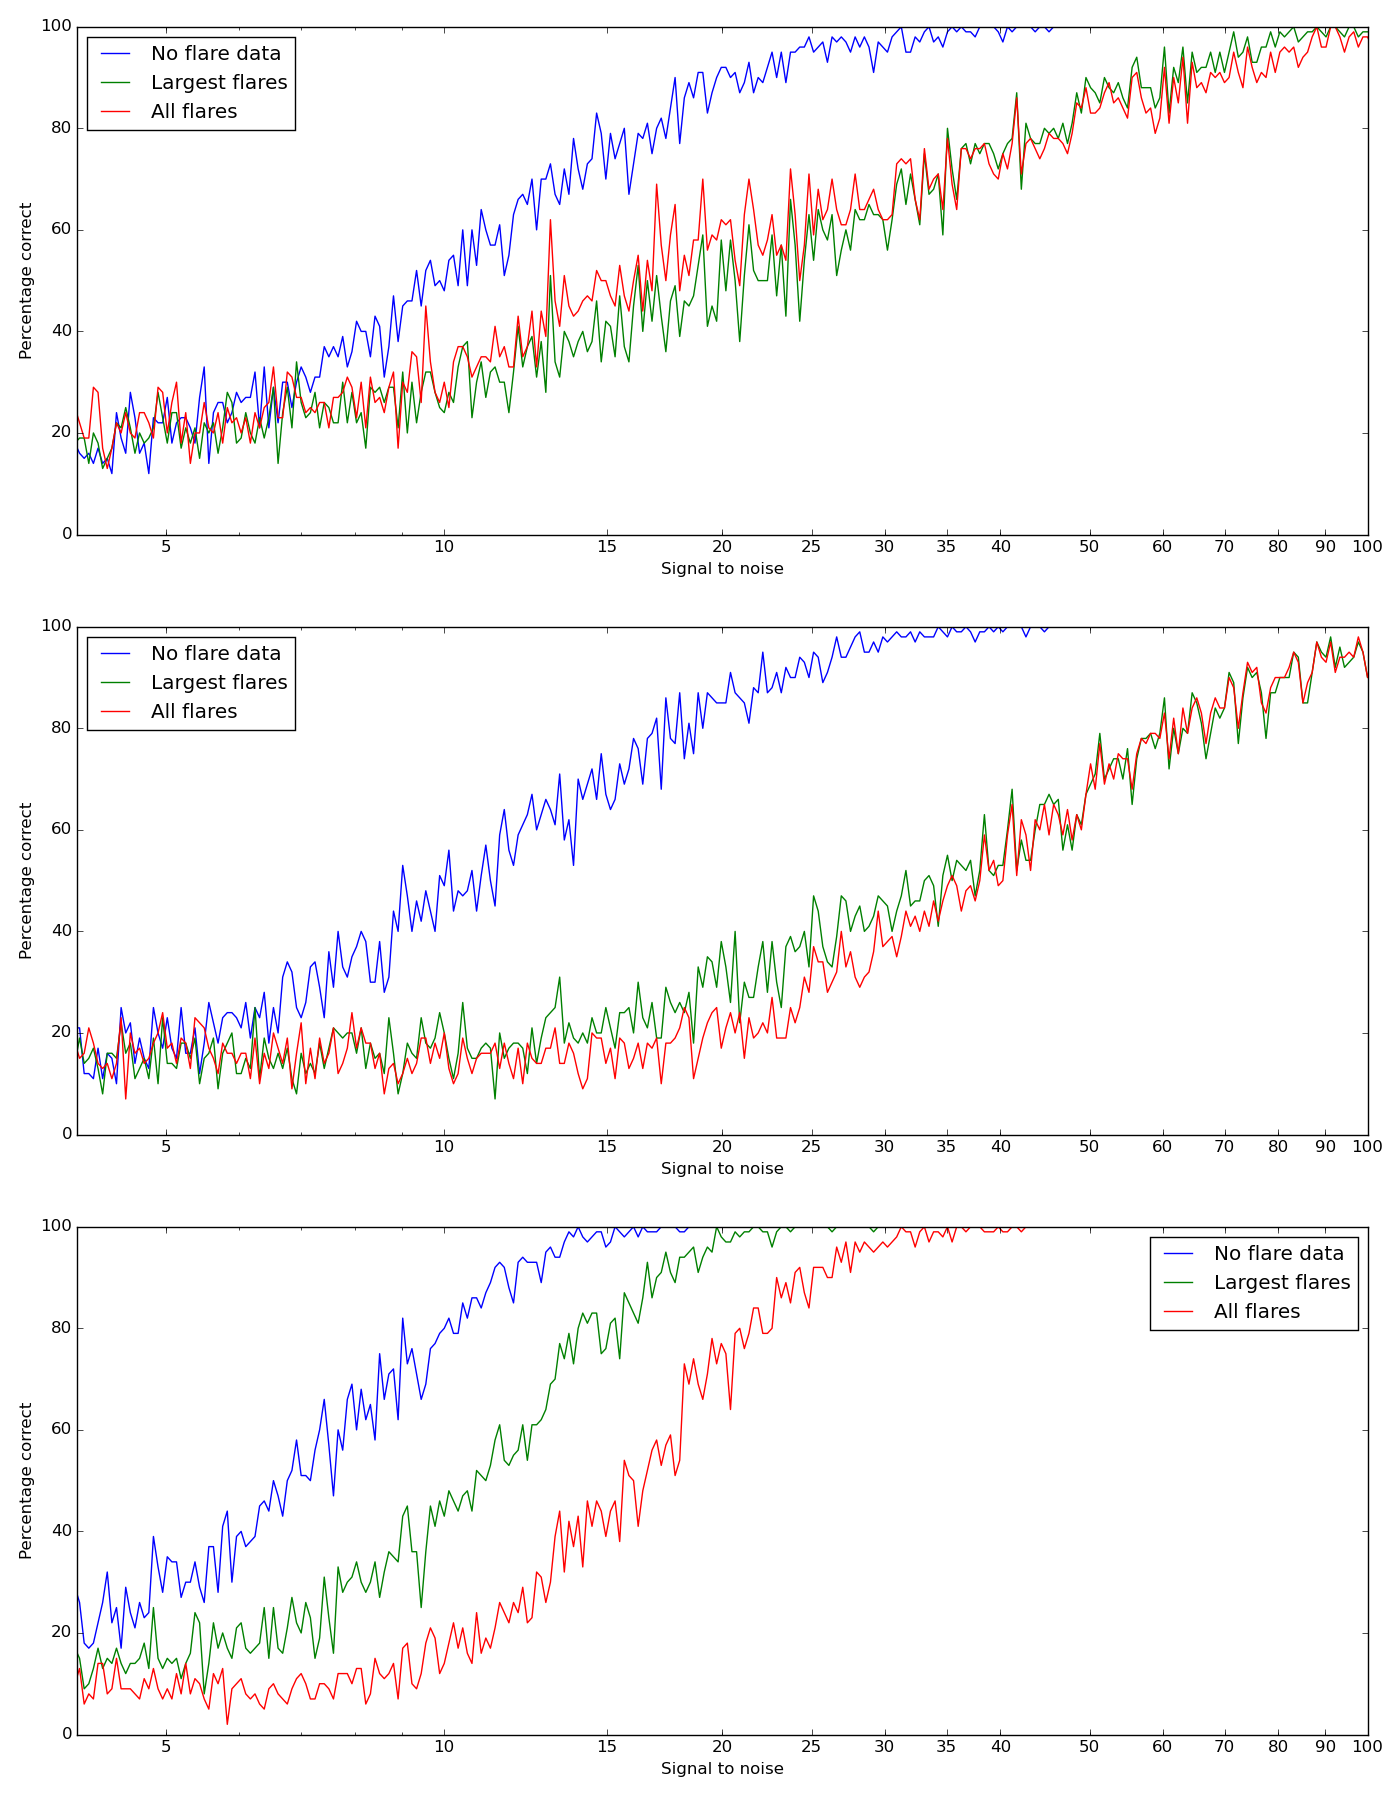
\includegraphics[scale=0.25]{Figures/Np80.png} \\
\end{center}
\caption{This figure shows the percentage of the correctly recovered period of 80 days as the strongest peak with
  various levels of SNR and adding various levels of simulated flare data, the blue plot for no flare data. the green
  plot with the four largest flare data (up to the January 2014) and the red plot the flare data clipped in Section
  \ref{section:harpsper} as having equivalent width greater than 1 standard deviation from the median in the original
  data to January 2014.  The topmost panel shows the results for an inclination of 30{\degree}, the middle panel that
  for 60{\degree} and the bottom panel for 90{\degree}.}
\protect\label{fig:noiseresults}
\end{figure}

It was of interest to note the impact of the rotation period on these results, in Fig. \ref{fig:noiseresults60} is shown
effectively the same data as Fig. \ref{fig:noiseresults}, but with a period of 60 days instead of 80 days. It was
noticeable how this performed significantly better than the 80-day period, closer to the 82.6-day period calculated for
\prox. Further reductions in the period improved the recovery still further, in a relationship apparently better than
linear (although many more simulations, in terms of numbers of runs and length of periods, would be required to
establish this with accuracy), lending weight to the contention that the spectroscopic line measurements are likely to
prove of more value with stars with a faster rotation period than \prox.

\begin{figure}[!htbp]
\begin{center}
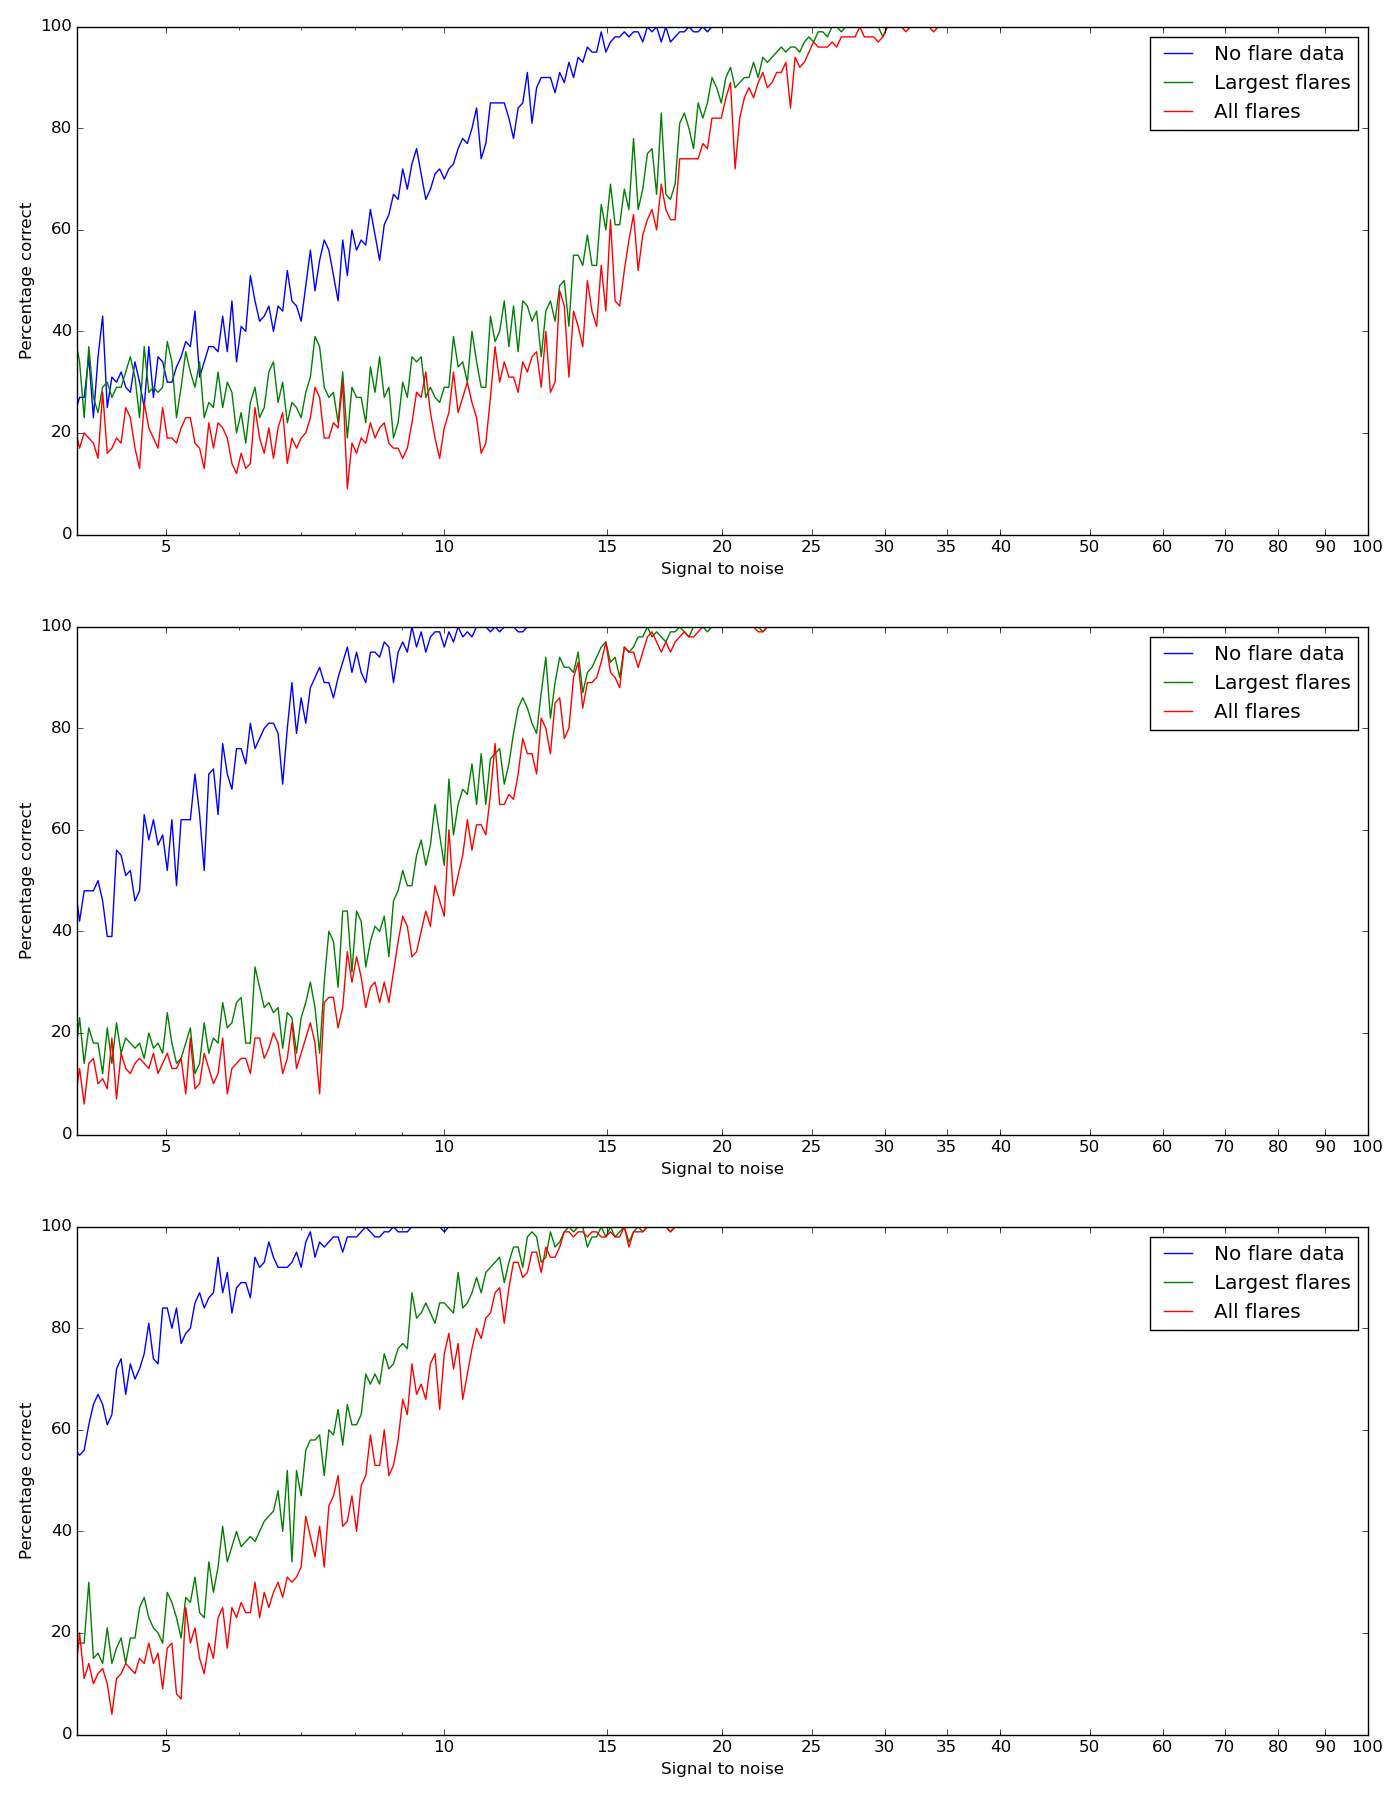
\includegraphics[scale=0.25]{Figures/Np60.png} \\
\end{center}
\caption{This figure is effectively the same as Fig. \ref{fig:noiseresults}, but from a starting period of 60 rather
  than 80 days, showing the significant improvement in the recovery rates with the shorter period.}
\protect\label{fig:noiseresults60}
\end{figure}

Some of the false positives from these simulations were noted and in quite a few cases it was noticed that periods close
to 116.6 days reported in \citet[Table 3]{suarezmascareno15} appeared as one of the prominent peaks in the modelling
results. An example is shown in Fig. \ref{fig:rec116}. This period is clearly an artefact of the observation times,
which were copied from the Original Set of {\harps} data for use in the model. \examrevision{This is further confirmed
  by \examrevisiona{periods close to this} being observed in the window function for those observation times as previously shown in
  Fig. \ref{fig:harpswfos}.}

\begin{figure}[!htbp]
\begin{center}
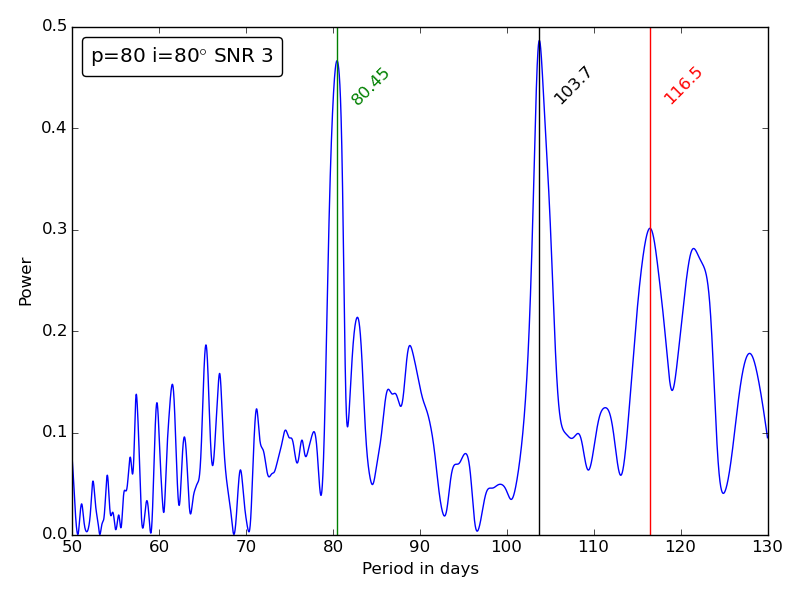
\includegraphics[scale=0.4]{Figures/badeg.png} \\
\end{center}
\caption{Example of a periodogram from the modelling simulations after adding noise which returns a peak close to 116.6
days.This was from a case where no flare data was added, to a model based on a period of 80 days, an inclination given
of 80{\degree} and a SNR of 3. Here 116.5 days appears as the third-strongest peak (highlighted in red). This example
gives the strongest peak as 103.7 days, marked in black and the correct period as 80.45 days, marked in green.}
\protect\label{fig:rec116}
\end{figure}

\chapter{Discussion}
\protect\label{chapter:discussion}
\lhead{Chapter \ref{chapter:discussion} \emph{Discussion}}

It is clear that the period of 82.6 $\pm$ 0.1 days given by the photometric results for {\asas} and confirmed by {\hst}
in Chapter \ref{chapter:photometry} must be the rotation period of \prox, in line with \citet{benedict98} and confirmed
by \citet{kiraga07}. There is a near-zero FAP value against 82.6 days and all the Lomb-Scargle routines which were tried
gave exactly the same result with identical periodograms (apart from allowances for scaling of the power which differed
between the routines). The experiments in Section \ref{section:asasfap} with taking subsets of the data and noting the
changes in FAP and the standard deviation of the error, with only limited extrapolation of the chart in
Fig. \ref{fig:asasprop}, give confidence in assigning the error bar on this period as being no more than 0.1 days.

It was not possible to obtain as clear-cut results from spectroscopic methods involving analysis of the {\ha} peak of
the {\prox} spectra, in terms of returning the period at all, obtaining a clear-cut topmost peak in the periodograms or
obtaining a reasonable error bar. As can be seen in the summary in Table \ref{table:perftable} or the full results in
Appendix \ref{chapter:pgramdetail}, the Peak Ratio method appears to perform significantly better, in terms of rate of
recovery of the correct period, than the Equivalent Width method, with skewness and kurtosis methods somewhere in
between. The results are of the same kind of order as the performance illustrated in Fig. \ref{fig:asasprop}, for
similar numbers of observations, but clearly cannot be used, standing alone, to compute the rotation period. Clipping high
equivalent width observations, or binning to various periods can improve some results, but not in any consistent way and
only seem to have an effect on Equivalent Width and Peak Ratio measurements, not with skewness and kurtosis
measurements, to which these made little difference.

There is also a strong peak of 106.3 $\pm$ 0.1 days on the {\asas} results and seen in some of the spectroscopic results
and the modelling, but not seen in the {\hst} results. This period would appear to be a ``beat'' between the rotation
period and an Earth year, which would not affect the {\hst} results, which are far less constrained by the time of
year. There is also a strong peak of 77.8 days on the {\hst} results which is not seen in the other results. Possibly
this is an alias or similar ``beat'' induced by the {\hst} observation times.

It has proved possible to reproduce the 116.6 days of \citet[Table 3]{suarezmascareno15} in both the treatments of
Equivalent Width and {\ha} Index and in some of the other variants of the handling of those, together with periodograms
taken from the skewness and kurtosis. However, this peak is the fifth strongest in the periodograms if the period search
is extended to 40 days and disappears if any kind of selection or binning is made from the data or if additional data
from 2016 is included. In addition, it was noticed that some of the modelling results (see Section
\ref{section:addflares}) also gave periods close to 116.6 days from the same observation times as in the {\harps}
data. From this analysis, this would clearly have to be discounted as a false positive, almost certainly an artefact of
the observation times.

Limiting the portion of the spectrum examined to just the {\ha} line of \prox, even with the instrumental stability of
{\harps} was proven to be less useful than {\asas} ground-based photometry for the recovery of period. A future line of
investigation which might be worth considering is that of combining fluxes from various magnetic/activity sensitive
lines in various spectral orders to re-evaluate the Composite Spectral Index referred to in \citet{hall99} and
\citet{hall00}. This was very briefly explored in the context of the examination of the TiO line and the He-6678 lines
described in Appendix \ref{chapter:tioline}, but a full treatment would require analysis of the prominent lines from all
the spectral orders.

It was possible to reproduce the variations in Equivalent Width seen in {\prox} using the DoTS model and show that the
recovery of the rotation period has validity. However, even with extensive experimentation, including relatively extreme
values for the various parameters for limb-darkening and contrast or extreme distributions of plage, it was not possible
to model the observed variations in Peak Ratio found either in the {\uves} or {\harps} data with a symmetric flux
profile. It is clear that the variations in the two \horn s that are purely due to Doppler shift from the rotational
velocity are not large; with a radius of 0.141 Solar \citep{demory09} and assuming a period of the order of 80 days the
rotational velocity is at most 90 m/s yielding a Doppler shift of at most 0.003{\AA} in the {\ha} line between the
extremes of the disk and the centre, far too low to reproduce the variations in the {\ha} line profile as as illustrated
in Fig. \ref{fig:harpsfirstha} for which the Peak Ratios were calculated as 0.997 $ \pm $ 0.018 (see Table
\ref{table:ewtabfirst}). The best standard deviation on a Peak Ratio close to 1.0 which could be obtained from the
models was $2{\times}10^{-5}$ or $2{\times}10^{-4}$ with very extreme plage distributions. This was not surprising due
to the lack of Doppler broadening of the line profile. However, more success with Peak Ratios was achieved by selecting
asymmetric flux profiles, as seen in Section \ref{section:vertvels}, suggesting that some additional net vertical
velocity may account for the observed behaviour of \prox, although this was a crude experiment as DoTS does not permit
this additional component to be properly varied according to the line of sight.

What was clear from the models was the way in which period recovery was adversely affected by the inclination and
improved as the rotation period was decreased, this is demonstrated by the results obtained in Section
\ref{section:addflares} and samples shown in Fig. \ref{fig:noiseresults} and Fig. \ref{fig:noiseresults60}. This at
least suggests that deducing the rotation period by photometric measurements may become increasingly feasible for faster
rotating stars.

It is probably naive to expect the plage configurations to be comparatively unchanged over such a long rotation period
as that for {\prox} and basing the models on this assumption is unlikely to reflect the observed variations
correctly. More importantly, it is also clear that the model of static plage and spots supported by DoTS cannot
accurately reproduce the observed variations in the Peak Ratios. Likewise it cannot reproduce the range of phenomena which
adversely affects obtaining periodicity from the Equivalent Widths.

This, together with the experiment with adding the effect of a net vertical velocity to the flux profiles to the DoTS
model showed some improvement in the variation of the Peak Ratios, but as noted this cannot be a proper model as it does
not reflect the variation of the vertical component towards the edge. Also it does not adversely effect the Equivalent
Width measure. This points to the need for a properly-constructed 3D model including vertical processes to properly
understand the behaviour of \prox.

In \citet{mohanty02} and \citet{mohanty03}, where the activity of late \rdwarf s is found to be less closely tied to the
rotation period for earlier type stars the authors propose a ``turbulent dynamo'' as the source of the activity, for
which a 3D model is required.

%A variety of phenomena in the literature were considered for this \paperorthesis. Also such a model ought to cater the
%possibility of Ellerman Bombs as described by Ellerman (1917) and recently discussed in \citet{rutten13} and
%\citet{vissers15} and \citet{rutten16} as particularly affecting the {\ha} line.
% These however were all treatments of the Sun. Again, this probably would not apply to {\prox} as they relate to much
% higher temperatures, in the range 10,000K to 20,000K, which would be very much less frequent with {\prox} and are
% explicitly stated to be a photospheric phenomenon.
%Another feature to be catered for in a more comprehensive model would be the possibility of prominence and plage
%activity as discussed by \citet{eibe98} for RE~1816+541. However this is a rapidly-rotating star, of the order of 12
%hours, rather than the 82 days of \prox. Also the literature such as \citet{skelly09}, building on earlier work such as
%\citet{donati99}, \citet{dunstone06} and \citet{colliercameron89} discusses the possibility of slingshot
%prominences. These however focus on K-dwarfs and appear to be associated with strong magnetic fields which would not be
%expected with a slow rotator such as \prox, although possibly the dynamo discussed in \citet{yadav16} may provide a clue
%to this.

In \citet{leenaarts12} a successful 3D MHD simulation was performed for the Sun. Also work on seismic shock waves has
been undertaken for example in \citet{donea06}. Similar conclusions are reached by \citet{rauscher06} as an explanation
for H, K and Ca line asymmetry, however these were for earlier type of stars than \prox, of type K7 to M5, for which
{\ha} is in absorption. The \horn s shown in fig. 2 in that paper have the red {\horn} smaller than the blue {\horn} as
opposed to {\prox} as shown in Fig. \ref{fig:harpsfirstha}, for which it is in most cases the other way round. The
authors suggest that this effect is caused by slowly-decelerating motion toward the observer which does not fall back
ballistically away from the observer which would therefore be blue-shifted and hence enhance the blue \horn. With \prox,
it might be a similar effect is taking place but the self-absorption portion is blue-shifted which would be inverted to
resemble a red shift.

%{\FirstP} finally noted the work on chromospheres in the review of \citet[Section VII]{linsky80} considering systematic
%chromospheric flow patterns. Linsky mostly considers Ca lines, but that review cites \citet{athay70} which particularly
%considers {\ha} and also \citet{athay70a}. These papers and others argue that vertically propagating shock waves can
%account for the red and blue asymmetries observed in various lines. In \citet{shkolnik03}, the authors build on this
%work to suggest that planets would induce such chromospheric activity on HD 179949 (an F8V star). The presence of the
%red and blue asymmetries in the {\ha} line on {\prox} as {\Firstp} observed does suggest this as a possible line of
%enquiry to build into new models. Somewhat similar to this is the discussion of line asymmetry of H, K and Ca lines in
%\citet{rauscher06}. In section 4.2 of
%that paper the authors suggest that line asymmetry is caused by a slowly-decelerating motion toward the observer which
%does not fall back ballistically away from the observer which would therefore be blue-shifted and hence enhance the blue
%\horn. On the other hand with \prox, it might be a similar effect is taking place but the self-absorption portion is
%blue-shifted which would be inverted to resemble a red shift.

%Future directions for {\prox} would therefore be to develop models to simulate some of these effects and attempt to
%relate them to the observed variations, particularly in the Peak Ratio. As for the measurements based on the {\ha} line
%and probably other lines, whilst {\Firstp} consider that they are currently less powerful than photometry for {\prox} in
%isolation, they may well be useful for other stars with a smaller rotation period whose Doppler variations in the
%morphology of the {\ha} and other lines dominate the effects.

\chapter{Conclusions}
\protect\label{chapter:conclusions}
\lhead{Chapter \ref{chapter:conclusions} \emph{Conclusions}}

This {\paperorthesis} has set out to study measurements of periodicity via measurements of the {\ha} line in particular
and focusing on \prox.

A study of photometric measurements from {\asas} and {\hst} produced clear evidence of a rotation period of 82.6 $\pm$
0.1 days with negligible FAP. This produced a benchmark from which to evaluate spectroscopic measurements including that
of Equivalent Width and the virtually identical {\ha} Index, which were applied to the {\ha} line to demonstrate that
they did not prove able, in terms of reliable recovery of the period at all or with an acceptable error bar, to deliver
a result in isolation, certainly as far as {\prox} is concerned. The measurement of lines presented in this
\paperorthesis, the Peak Ratio, appears to be consistently better than other measurements and is particularly suitable
for {\ha} line profiles such as that for \prox, which have a ``horned'' appearance with two \horn s around a relatively
unchanging central minimum.

A look at simple 2D models enabled the validity of the method to be established for Equivalent Widths, but not for Peak
Ratios, in the face of varying SNR levels and simulated flares. However the models were ``too good'' for Equivalent
Width whilst not good enough for Peak Ratios. The need for a more sophisticated 3D model with vertical motion is clear
if the activity in \prox, probably other late \rdwarf s with lower rotation period but relatively high activity, are to
be understood.

In this process a recent assessment of the rotation period of {\prox} as 116.6 days was discounted as a false positive.




%----------------------------------------------------------------------------------------
%	THESIS CONTENT - APPENDICES
%----------------------------------------------------------------------------------------

\addtocontents{toc}{\vspace{2em}} % Add a gap in the Contents, for aesthetics

\appendix % Cue to tell LaTeX that the following 'chapters' are Appendices

% Include the appendices of the thesis as separate files from the Appendices folder
% Uncomment the lines as you write the Appendices

\chapter{Full periodogram results} % Main appendix title
\protect\label{chapter:pgramdetail}
\lhead{Appendix \ref{chapter:pgramdetail}. \emph{Periodogram details}}

In this appendix the complete results for the periodicity studies with various treatments of the data and Python
routines are presented.

\section{Equivalent Widths}
\protect\label{section:appewtab}

The following tables, Table \ref{table:origewtaball} and \ref{table:fullewtaball}, present all the periodogram
calculations with the three Python routines employed, with the Original Set of {\harps} data to January 2014 and the
Full Set to March 2016 respectively. The Equivalent Widths are calculated with the Original Set to highlight that the 116-day
period found in \citet{suarezmascareno15} is also returned with those, but not with the Full Set to January 2014.

\begin{table}[!htbp]
\centering
\scalebox{0.75}{
\begin{tabular}{|l|l|l|r|r|r|r|r|}
\hline
\textbf{Treatment}&\textbf{Points}&\textbf{Routine}&\textbf{Peak 1}&\textbf{Peak 2}&\textbf{Peak 3}&\textbf{Peak 4}&\textbf{Peak 5}\\\hline
None & \multirow{3}{*}{260} & \scipy & 116.2 & \textit{41.4} & 52.1 & 46.2 & 48.9 \\
 && \astroml & 44.9 & 57.6 & 59.4 & 104.2 & 84.4 \\
 && \gatspy & 49.1 & \textit{41.4} & 49.9 & 57.0 & 116.3 \\\hline
Clipped 1$\sigma$ & \multirow{3}{*}{237} & \scipy & 118.4 & 57.7 & 106.8 & 105.3 & 44.9 \\
 && \astroml & 45.0 & 51.2 & 57.7 & 47.4 & 84.5 \\
 && \gatspy & 44.9 & 118.4 & 57.8 & 107.2 & 46.4 \\\hline
Binned & \multirow{3}{*}{57} & \scipy & \textit{41.4} & 53.2 & 110.5 & 62.6 & 116.1 \\
1 day && \astroml & 115.5 & 87.7 & 71.1 & 59.4 & 40.0 \\
 && \gatspy & \textit{41.4} & 53.2 & 110.5 & 62.6 & 49.9 \\\hline
Binned & \multirow{3}{*}{89} & \scipy & \textit{41.4} & 110.4 & 53.1 & 49.0 & 49.9 \\
0.5 day && \astroml & 45.0 & 115.0 & 59.4 & 110.3 & \textbf{82.6} \\
 && \gatspy & \textit{41.4} & 49.0 & 57.0 & 59.3 & 49.9 \\\hline
Clipped 1$\sigma$ & \multirow{3}{*}{55} & \scipy & 45.0 & 59.5 & 71.4 & 89.0 & 109.7 \\
binned && \astroml & 59.5 & 45.0 & 71.3 & 49.9 & 51.2 \\
1 day && \gatspy & 45.0 & 59.5 & 71.4 & 89.0 & 107.7 \\\hline
Clipped 1$\sigma$ & \multirow{3}{*}{83} & \scipy & 45.0 & 59.5 & 51.2 & 71.3 & 117.3 \\
binned && \astroml & 45.0 & 51.2 & 40.0 & 59.5 & 57.9 \\
0,5 day && \gatspy & 45.0 & 59.5 & 51.3 & 71.5 & 117.3 \\\hline
Residuals & \multirow{3}{*}{260} & \scipy & 116.2 & \textit{41.4} & 48.9 & 52.1 & 53.0 \\
 && \astroml & 45.0 & 59.4 & 57.6 & 84.3 & 104.2 \\
 && \gatspy & 49.1 & \textit{41.4} & 49.9 & 57.0 & 116.3 \\\hline
\end{tabular}}
\caption{This table shows the 5 highest peaks from the periodograms for Equivalent Widths with various treatments of the
  Original Set of data to January 2014. Highlighted in bold are periods within 2\% of 82.6 days and in italics periods within 2\% of 41.3 days.}
\protect\label{table:origewtaball}
\end{table}

\begin{table}[!htbp]
\centering
\scalebox{0.75}{
\begin{tabular}{|l|l|l|r|r|r|r|r|}
\hline
\textbf{Treatment}&\textbf{Points}&\textbf{Routine}&\textbf{Peak 1}&\textbf{Peak 2}&\textbf{Peak 3}&\textbf{Peak 4}&\textbf{Peak 5}\\\hline
None & \multirow{3}{*}{316} & \scipy & 49.0 & \textit{41.4} & 62.6 & 56.8 & 53.2 \\
 && \astroml & 114.6 & 123.2 & 108.0 & \textbf{83.1} & 91.8 \\
 && \gatspy & 59.2 & 49.0 & 62.6 & 56.9 & \textit{41.4} \\\hline
Clipped 1$\sigma$ & \multirow{3}{*}{287} & \scipy & 122.2 & 108.0 & \textbf{83.1} & 90.2 & 99.1 \\
 && \astroml & 123.1 & 114.9 & 107.8 & \textbf{83.1} & 91.8 \\
 && \gatspy & 122.5 & 108.0 & 59.1 & 48.1 & 50.1 \\\hline
Clipped & \multirow{3}{*}{277} & \scipy & 108.0 & 122.0 & \textbf{83.0} & 90.0 & 120.1 \\
To 3.8 EW && \astroml & 123.3 & 114.7 & 107.9 & \textbf{83.2} & 87.0 \\
 && \gatspy & 108.0 & 122.2 & 58.1 & \textbf{83.1} & 89.9 \\\hline
Binned & \multirow{3}{*}{93} & \scipy & \textit{41.4} & 49.0 & 62.6 & 53.3 & 59.2 \\
1 day && \astroml & 123.0 & 114.5 & 91.7 & 101.1 & 107.8 \\
 && \gatspy & \textit{41.4} & 59.2 & 49.0 & 62.6 & 53.3 \\\hline
Binned & \multirow{3}{*}{143} & \scipy & 49.0 & 59.2 & \textit{41.4} & 62.6 & 56.8 \\
0.5 day && \astroml & 114.5 & 123.2 & 91.8 & \textbf{83.1} & 108.0 \\
 && \gatspy & 59.2 & 49.0 & \textit{41.4} & 62.6 & 56.8 \\\hline
Clipped 1$\sigma$ & \multirow{3}{*}{89} & \scipy & 114.9 & 123.3 & 108.0 & 87.0 & \textbf{83.2} \\
binned && \astroml & 114.8 & 123.2 & 91.7 & 107.7 & 87.0 \\
1 day && \gatspy & 114.9 & 123.3 & 108.0 & 87.0 & \textbf{83.2} \\\hline
Clipped & \multirow{3}{*}{85} & \scipy & 114.8 & 108.0 & 123.4 & 86.9 & \textbf{83.1} \\
To 3.8 EW && \astroml & 114.6 & 123.2 & 107.7 & 91.7 & 86.9 \\
binned 1 day && \gatspy & 114.8 & 108.0 & 123.4 & 86.9 & \textbf{83.1} \\\hline
Clipped 1$\sigma$ & \multirow{3}{*}{129} & \scipy & 114.8 & 123.4 & 108.1 & \textbf{83.2} & 87.0 \\
binned && \astroml & 114.8 & 123.1 & 91.9 & 107.7 & \textbf{83.2} \\
0.5 day && \gatspy & 114.9 & 123.4 & 108.0 & \textbf{83.2} & 54.9 \\\hline
Clipped & \multirow{3}{*}{122} & \scipy & 114.7 & 108.1 & 123.4 & 86.9 & \textbf{83.2} \\
To 3.8 EW && \astroml & 114.7 & 123.3 & 107.9 & 92.0 & 87.0 \\
binned 0.5 day && \gatspy & 114.8 & 108.0 & 123.4 & 86.9 & \textbf{83.2} \\\hline
Residuals & \multirow{3}{*}{316} & \scipy & 49.0 & \textit{41.4} & 62.6 & 56.8 & 53.3 \\
 && \astroml & 114.6 & 123.2 & 108.0 & \textbf{83.1} & 91.8 \\
 && \gatspy & 59.2 & 49.0 & 62.6 & 56.9 & \textit{41.4} \\\hline
\end{tabular}}
\caption{This table shows the 5 highest peaks from the periodograms for Equivalent Widths with various treatments of the
  Full Set of data to March 2916. Highlighted in bold are periods within 2\% of 82.6 days and in italics periods within
  2\% of 41.3 days.}
\protect\label{table:fullewtaball}
\end{table}

In these tables where spectra are clipped as having Equivalent Width over one standard deviation above the median, this
is to the values given in Table \ref{table:ewtabfirst}, i.e. 3.8 for the Original Set to 2014 and 4.2 for the Full Set
to 2016.

The residual Equivalent Widths are calculated by dividing by the mean of the 5 spectra with the smallest {\ha}
Equivalent Widths. These spectra were ones timed at 5 April 2011 UTC 03:26:33 (the lowest), 16 March 2006 UTC 06:37:59,
14 March 2007 UTC 07:28:29, 8 April 2011 UTC 06:28:17 and 22 April 2011 UTC 05:07:46.

\section{{\ha} Index measurement}
\protect\label{section:apphaitab}

In Table \ref{table:bothhaitable} is shown the results for all three Python routines used evaluating the {\ha} Index.
These are calculated with the Original Set of data to 2014 as well as the Full Set to 2016 to highlight that the 116-day
period found in \citet{suarezmascareno15} with the Original Set, but not with the Full Set to January 2014.

\begin{table}[!htbp]
\centering
\scalebox{0.75}{
\begin{tabular}{|l|l|r|r|r|r|r|}
\hline
\textbf{Data}&\textbf{Routine}&\textbf{Peak 1}&\textbf{Peak 2}&\textbf{Peak 3}&\textbf{Peak 4}&\textbf{Peak 5}\\\hline
Set to 2014 & \scipy & 116.2 & 41.4 & 52.1 & 48.9 & 53.0 \\
 & \astroml & 45.0 & 51.2 & 57.6 & 84.5 & 116.6 \\
 & \gatspy & 49.1 & 41.4 & 49.9 & 57.0 & 116.3 \\\hline
Full Set & \scipy & 49.0 & 41.4 & 62.6 & 56.8 & 53.3 \\
 & \astroml & 123.2 & 114.7 & 107.9 & 83.1 & 87.0 \\
 & \gatspy & 59.2 & 49.0 & 62.6 & 56.9 & 41.4 \\\hline
\end{tabular}}
\caption{This table shows the 5 highest peaks from the periodograms for the Original and Full Sets of Data.}
\protect\label{table:bothhaitable}
\end{table}

\section{{\ha} Peak Ratio measurments}
\protect\label{section:appprtab}

The following tables, Table \ref{table:origprtaball} and \ref{table:fullprtaball}, present all the periodogram
calculations with the three Python routines employed, with the Original Set of {\harps} data to January 2014 and the
Full Set to March 2016 respectively. The Peak Ratios are calculated with the Original Set to highlight that the 116-day
period found in \citet{suarezmascareno15} for the {\ha} Index measurement (and also with the Equivalent Widths, see
Section \ref{section:appewtab} is not returned with this measurement.

\begin{table}[!htbp]
\centering
\scalebox{0.75}{
\begin{tabular}{|l|l|l|r|r|r|r|r|}
\hline
\textbf{Treatment}&\textbf{Points}&\textbf{Routine}&\textbf{Peak 1}&\textbf{Peak 2}&\textbf{Peak 3}&\textbf{Peak 4}&\textbf{Peak 5}\\\hline
None & \multirow{3}{*}{260} & \scipy & \textit{41.9} & 92.4 & \textbf{81.1} & 49.7 & 44.1 \\
 && \astroml & 80.0 & 103.9 & 92.5 & 49.2 & 45.5 \\
 && \gatspy & \textbf{81.0} & \textit{41.9} & 92.4 & 103.9 & 44.1 \\\hline
Clipped 1$\sigma$ & \multirow{3}{*}{237} & \scipy & \textit{41.9} & \textbf{81.3} & 49.8 & 92.1 & 44.1 \\
 && \astroml & 49.9 & \textit{41.9} & 91.9 & 101.5 & 58.1 \\
 && \gatspy & \textbf{81.2} & \textit{41.9} & 49.8 & 92.2 & 44.1 \\\hline
Binned & \multirow{3}{*}{57} & \scipy & \textbf{82.2} & 61.0 & 80.9 & 49.6 & \textit{40.6} \\
1 day && \astroml & 71.1 & 115.2 & 80.0 & 91.8 & 123.2 \\
 && \gatspy & \textbf{82.3} & 61.0 & 49.4 & \textbf{81.0} & \textit{40.6} \\\hline
Binned & \multirow{3}{*}{89} & \scipy & 122.2 & 120.3 & \textbf{82.9} & 79.7 & 108.4 \\
0.5 day && \astroml & 80.5 & 91.9 & 115.0 & 104.0 & 109.6 \\
 && \gatspy & 122.1 & \textbf{83.0} & 79.8 & 108.4 & 78.1 \\\hline
Clipped 1$\sigma$ & \multirow{3}{*}{55} & \scipy & \textbf{82.2} & 61.1 & \textit{40.5} & \textbf{81.0} & 115.8 \\
binned && \astroml & 108.0 & 71.2 & 80.0 & 57.1 & 65.5 \\
1 day && \gatspy & \textbf{82.2} & 61.1 & \textit{40.5} & \textbf{81.0} & 49.3 \\\hline
Clipped 1$\sigma$ & \multirow{3}{*}{83} & \scipy & 122.2 & 120.2 & \textbf{82.6} & 108.3 & 78.2 \\
binned && \astroml & 108.8 & 57.8 & 47.3 & 103.5 & 54.4 \\
0,5 day && \gatspy & 122.2 & 120.5 & \textbf{82.7} & 108.3 & 79.7 \\\hline
Residuals & \multirow{3}{*}{260} & \scipy & \textit{41.9} & \textit{41.4} & 49.7 & 92.4 & 44.2 \\
 && \astroml & 45.4 & 80.0 & \textbf{84.1} & 92.6 & 49.2 \\
 && \gatspy & \textit{41.9} & 45.5 & 49.8 & \textit{41.4} & 80.9 \\\hline
\end{tabular}}
\caption{This table shows the 5 highest peaks from the periodograms for Peak Ratios with various treatments of the
  Original Set of data to January 2014. Highlighted in bold are periods within 2\% of 82.6 days and in italics periods
  within 2\% of 41.3 days.}
\protect\label{table:origprtaball}
\end{table}

\begin{table}[!htbp]
\centering
\scalebox{0.75}{
\begin{tabular}{|l|l|l|r|r|r|r|r|}
\hline
\textbf{Treatment}&\textbf{Points}&\textbf{Routine}&\textbf{Peak 1}&\textbf{Peak 2}&\textbf{Peak 3}&\textbf{Peak 4}&\textbf{Peak 5}\\\hline
None & \multirow{3}{*}{316} & \scipy & 121.7 & 123.3 & \textbf{83.0} & 114.6 & 90.1 \\
 && \astroml & 60.6 & 52.1 & 49.1 & 56.9 & 57.9 \\
 && \gatspy & 121.8 & 49.9 & 114.7 & \textbf{83.0} & \textit{42.0} \\\hline
Clipped 1$\sigma$ & \multirow{3}{*}{287} & \scipy & 122.3 & 91.8 & \textbf{83.0} & 115.0 & \textit{42.0} \\
 && \astroml & 60.8 & 73.0 & 102.0 & 79.5 & 56.8 \\
 && \gatspy & 122.5 & 58.1 & 47.5 & \textbf{83.0} & 91.7 \\\hline
Clipped & \multirow{3}{*}{277} & \scipy & 122.2 & 114.9 & 91.8 & \textbf{82.9} & 49.8 \\
To 3.8 EW && \astroml & 101.8 & 73.1 & 114.3 & 79.3 & 91.2 \\
 && \gatspy & 122.5 & 49.9 & 58.0 & 115.0 & 91.8 \\\hline
Binned & \multirow{3}{*}{93} & \scipy & \textbf{82.2} & \textit{40.6} & 51.1 & 63.6 & 66.8 \\
1 day && \astroml & 91.6 & 60.9 & 87.0 & 79.3 & 122.0 \\
 && \gatspy & \textbf{82.2} & \textit{40.6} & 51.1 & 63.6 & 48.0 \\\hline
Binned & \multirow{3}{*}{143} & \scipy & 120.4 & 121.7 & \textbf{82.3} & 107.6 & 117.5 \\
0.5 day && \astroml & 54.4 & 60.6 & 64.1 & 73.0 & 67.3 \\
 && \gatspy & 120.7 & \textbf{82.3} & 107.5 & 117.4 & 80.0 \\\hline
Clipped 1$\sigma$ & \multirow{3}{*}{89} & \scipy & \textit{40.5} & 80.9 & 48.1 & 116.7 & 51.1 \\
binned && \astroml & 114.8 & 91.4 & 122.1 & 122.7 & 107.4 \\
1 day && \gatspy & \textit{40.5} & 80.9 & 48.1 & 119.9 & 116.7 \\\hline
Clipped & \multirow{3}{*}{85} & \scipy & \textit{40.5} & 80.9 & 116.4 & \textbf{81.8} & 48.0 \\
To 3.8 EW && \astroml & 114.3 & 59.8 & 54.5 & 121.9 & 107.1 \\
binned 1 day && \gatspy & \textit{40.5} & 80.9 & 116.5 & \textbf{81.9} & 48.0 \\\hline
Clipped 1$\sigma$ & \multirow{3}{*}{129} & \scipy & 121.8 & 120.4 & \textbf{82.4} & 107.7 & 117.3 \\
binned && \astroml & 60.8 & 73.0 & 69.0 & 91.2 & 54.4 \\
0.5 day && \gatspy & 120.8 & 121.3 & \textbf{82.4} & 107.6 & 117.3 \\\hline
Clipped & \multirow{3}{*}{122} & \scipy & 121.8 & 120.4 & \textbf{82.4} & 107.7 & 117.2 \\
To 3.8 EW && \astroml & 91.2 & 67.4 & 73.0 & 101.8 & 69.0 \\
binned 0.5 day && \gatspy & 120.7 & 121.3 & \textbf{82.4} & 107.6 & 117.2 \\\hline
Residuals & \multirow{3}{*}{316} & \scipy & 121.6 & 123.7 & 49.8 & 90.0 & \textbf{83.0} \\
 && \astroml & 60.6 & 73.1 & 79.6 & 65.0 & 57.0 \\
 && \gatspy & 121.7 & 49.9 & 123.7 & 58.0 & 47.5 \\\hline
\end{tabular}}
\caption{This table shows the 5 highest peaks from the periodograms for Peak Ratios with various treatments of the
  Full Set of data to March 2916. Highlighted in bold are periods within 2\% of 82.6 days and in italics periods within
  2\% of 41.3 days.}
\protect\label{table:fullprtaball}
\end{table}

In these tables the clipping, binning and calculation of residuals is exactly as described above for Equivalent Widths
in Section \ref{section:appewtab}.

\section{Skewness and Kurtosis measurements}
\protect\label{section:appkstab}

The following tables, Table \ref{table:origskewtaball} and \ref{table:origkurttaball} present the periodogram
calculations with the three Python routines employed, with the Original Set of {\harps} data to January 2014. Following
these the Tables \ref{table:fullskewtaball} and \ref{table:fullkurttaball} present the periodogram calculations for the
Full Set of data to March 2016.

As with the Equivalent Widths in Section \ref{section:appewtab}, the calculation is performed for the Original Set of data as
the 116-day period found in \citet{suarezmascareno15} again appears, even in this case after clipping, binning or both
is attempted.

\begin{table}[!htbp]
\centering
\scalebox{0.75}{
\begin{tabular}{|l|l|r|r|r|r|r|}
\hline
\textbf{Treatment}&\textbf{Routine}&\textbf{Peak 1}&\textbf{Peak 2}&\textbf{Peak 3}&\textbf{Peak 4}&\textbf{Peak 5}\\\hline
None & \scipy & 122.8 & 98.3 & 87.6 & 117.2 & 106.0 \\
 & \astroml & 87.7 & 116.8 & 105.5 & 122.4 & 79.7 \\
 & \gatspy & 87.7 & 116.8 & 105.5 & 122.4 & 79.7 \\\hline
Clipped 1$\sigma$ & \scipy & 98.2 & 122.9 & 65.3 & 71.3 & 59.7 \\
 & \astroml & 87.5 & 65.5 & 115.8 & 79.8 & 98.2 \\
 & \gatspy & 87.5 & 65.5 & 115.8 & 79.8 & 98.2 \\\hline
Binned & \scipy & 105.7 & 117.7 & 87.8 & 103.3 & 79.6 \\
1 day & \astroml & 105.7 & 117.7 & 87.8 & 103.3 & 48.8 \\
 & \gatspy & 105.7 & 117.7 & 87.8 & 103.3 & 48.8 \\\hline
Binned & \scipy & 105.8 & 87.7 & 117.3 & 79.6 & \textbf{81.2} \\
0.5 day & \astroml & 105.7 & 87.7 & 117.4 & 79.6 & \textbf{81.2} \\
 & \gatspy & 105.7 & 87.7 & 117.4 & 79.6 & \textbf{81.2} \\\hline
Clipped 1$\sigma$ & \scipy & 59.6 & 87.7 & 117.1 & 65.5 & 105.6 \\
binned & \astroml & 59.6 & 87.7 & 117.0 & 65.5 & 105.6 \\
1 day & \gatspy & 59.6 & 87.7 & 117.0 & 65.5 & 105.6 \\\hline
Clipped 1$\sigma$ & \scipy & 87.6 & 116.5 & 65.5 & 59.7 & 105.5 \\
binned & \astroml & 87.6 & 65.5 & 116.5 & 59.7 & 105.5 \\
0,5 day & \gatspy & 87.6 & 65.5 & 116.5 & 59.7 & 105.5 \\\hline
Residuals & \scipy & 71.8 & 73.8 & 57.7 & 93.0 & 98.4 \\
 & \astroml & 93.1 & \textbf{83.7} & 74.1 & 52.2 & 71.9 \\
 & \gatspy & 93.1 & \textbf{83.7} & 74.1 & 52.2 & 71.9 \\\hline
\end{tabular}}
\caption{This table shows the 5 highest peaks from the periodograms for Skewness with various treatments of the Original
  Set of data to January 2014. Highlighted in bold are periods within 2\% of 82.6 days and in italics periods within 2\% of
  to 41.3 days.}
\protect\label{table:origskewtaball}
\end{table}

\begin{table}[!htbp]
\centering
\scalebox{0.75}{
\begin{tabular}{|l|l|r|r|r|r|r|}
\hline
\textbf{Treatment}&\textbf{Routine}&\textbf{Peak 1}&\textbf{Peak 2}&\textbf{Peak 3}&\textbf{Peak 4}&\textbf{Peak 5}\\\hline
None & \scipy & 117.2 & 122.7 & 106.4 & 87.2 & 103.6 \\
 & \astroml & 116.7 & 80.9 & 87.3 & 105.2 & 103.7 \\
 & \gatspy & 116.7 & 80.9 & 87.3 & 105.2 & 103.7 \\\hline
Clipped 1$\sigma$ & \scipy & 117.2 & 87.3 & 59.6 & 65.4 & 122.5 \\
 & \astroml & 116.8 & 80.9 & 87.5 & 65.5 & 59.8 \\
 & \gatspy & 116.8 & 80.9 & 87.5 & 65.5 & 59.8 \\\hline
Binned & \scipy & 116.5 & 105.3 & 88.8 & 103.7 & 87.6 \\
1 day & \astroml & 116.4 & 105.3 & 103.8 & 88.8 & 87.6 \\
 & \gatspy & 116.4 & 105.3 & 103.8 & 88.8 & 87.6 \\\hline
Binned & \scipy & 116.6 & 87.5 & 88.4 & 105.4 & 80.5 \\
0.5 day & \astroml & 116.6 & 87.5 & 105.3 & 80.8 & 88.4 \\
 & \gatspy & 116.6 & 87.5 & 105.3 & 80.8 & 88.4 \\\hline
Clipped 1$\sigma$ & \scipy & 59.6 & 117.9 & 45.0 & 80.9 & 87.8 \\
binned & \astroml & 59.6 & 118.1 & \textbf{81.0} & 105.7 & 45.0 \\
1 day & \gatspy & 59.6 & 118.1 & \textbf{81.0} & 105.7 & 45.0 \\\hline
Clipped 1$\sigma$ & \scipy & 117.2 & 59.6 & 87.7 & 65.6 & 80.8 \\
binned & \astroml & 117.5 & 59.6 & 87.7 & 65.6 & \textbf{81.0} \\
0,5 day & \gatspy & 117.5 & 59.6 & 87.7 & 65.6 & \textbf{81.0} \\\hline
Residuals & \scipy & 117.6 & 106.6 & 103.5 & 74.0 & 51.4 \\
 & \astroml & 117.4 & \textbf{81.1} & 106.3 & 57.3 & 103.5 \\
 & \gatspy & 117.4 & \textbf{81.1} & 106.3 & 57.3 & 103.5 \\\hline
\end{tabular}}
\caption{This table shows the 5 highest peaks from the periodograms for Kurtosis with various treatments of the Original
  Set of data to January 2014. Highlighted in bold are periods within 2\% of 82.6 days and in italics periods within 2\%
  of 41.3 days.}
\protect\label{table:origkurttaball}
\end{table}

\begin{table}[!htbp]
\centering
\scalebox{0.75}{
\begin{tabular}{|l|l|r|r|r|r|r|}
\hline
\textbf{Treatment}&\textbf{Routine}&\textbf{Peak 1}&\textbf{Peak 2}&\textbf{Peak 3}&\textbf{Peak 4}&\textbf{Peak 5}\\\hline
None & \scipy & 121.9 & \textbf{83.4} & 60.0 & 79.1 & 106.4 \\
 & \astroml & \textbf{83.4} & 122.2 & 60.0 & 63.4 & 77.7 \\
 & \gatspy & \textbf{83.4} & 122.2 & 60.0 & 63.4 & 77.7 \\\hline
Clipped 1$\sigma$ & \scipy & 121.9 & 99.1 & 59.9 & \textbf{83.3} & 65.1 \\
 & \astroml & 59.9 & 63.3 & 77.8 & \textbf{83.3} & 113.5 \\
 & \gatspy & 59.9 & 63.3 & 77.8 & \textbf{83.3} & 113.5 \\\hline
Clipped & \scipy & 121.9 & 65.1 & 99.0 & \textbf{83.3} & 59.9 \\
To 3.8 EW & \astroml & 60.0 & 86.1 & 113.7 & 77.7 & 122.2 \\
 & \gatspy & 60.0 & 86.1 & 113.7 & 77.7 & 122.2 \\\hline
Binned & \scipy & 106.8 & 79.2 & 85.8 & 121.5 & 64.8 \\
1 day & \astroml & 106.8 & 79.2 & 85.8 & 121.6 & 64.8 \\
 & \gatspy & 106.8 & 79.2 & 85.8 & 121.6 & 64.8 \\\hline
Binned & \scipy & 79.2 & 85.8 & 106.7 & 60.0 & \textbf{83.4} \\
0.5 day & \astroml & 85.8 & 106.7 & 79.2 & 60.0 & \textbf{83.4} \\
 & \gatspy & 85.8 & 106.7 & 79.2 & 60.0 & \textbf{83.4} \\\hline
Clipped & \scipy & 59.7 & 71.9 & 85.9 & \textit{41.4} & 77.6 \\
1$\sigma$ & \astroml & 59.7 & 71.9 & 85.9 & \textit{41.4} & 107.0 \\
binned 1 day & \gatspy & 59.7 & 71.9 & 85.9 & \textit{41.4} & 107.0 \\\hline
Clipped & \scipy & 59.9 & 86.0 & 113.5 & 72.0 & 77.7 \\
1$\sigma$ & \astroml & 59.8 & 86.0 & 113.4 & 72.0 & 77.7 \\
binned 0.5 day & \gatspy & 59.8 & 86.0 & 113.4 & 72.0 & 77.7 \\\hline
Clipped & \scipy & 59.7 & 71.9 & 85.9 & 106.8 & 113.7 \\
To 3.8 EW & \astroml & 59.7 & 71.9 & 85.9 & 106.9 & 113.6 \\
binned 1 day & \gatspy & 59.7 & 71.9 & 85.9 & 106.9 & 113.6 \\\hline
Clipped & \scipy & 86.0 & 113.6 & 59.9 & 77.7 & 72.0 \\
To 3.8 EW & \astroml & 86.0 & 113.5 & 59.9 & 77.7 & 72.0 \\
binned 0.5 day & \gatspy & 86.0 & 113.5 & 59.9 & 77.7 & 72.0 \\\hline
Residuals & \scipy & 121.5 & 98.6 & 108.2 & 90.2 & 105.9 \\
 & \astroml & 108.2 & 121.8 & 105.8 & 90.1 & \textbf{83.4} \\
 & \gatspy & 108.2 & 121.8 & 105.8 & 90.1 & \textbf{83.4} \\\hline
\end{tabular}}
\caption{This table shows the 5 highest peaks from the periodograms for Skewness with various treatments of the Full
  Set of data to March 2016. Highlighted in bold are periods within 2\% of 82.6 days and in italics periods within 2\% of 41.3 days.}
\protect\label{table:fullskewtaball}
\end{table}

\begin{table}[!htbp]
\centering
\scalebox{0.75}{
\begin{tabular}{|l|l|r|r|r|r|r|}
\hline
\textbf{Treatment}&\textbf{Routine}&\textbf{Peak 1}&\textbf{Peak 2}&\textbf{Peak 3}&\textbf{Peak 4}&\textbf{Peak 5}\\\hline
None & \scipy & 122.8 & 86.8 & \textbf{83.1} & 114.4 & 79.4 \\
 & \astroml & 122.9 & 114.6 & 86.8 & 86.0 & \textbf{83.0} \\
 & \gatspy & 122.9 & 114.6 & 86.8 & 86.0 & \textbf{83.0} \\\hline
Clipped 1$\sigma$ & \scipy & 122.9 & 86.9 & 114.5 & 65.1 & \textbf{83.1} \\
 & \astroml & 114.7 & 86.9 & 122.9 & 86.1 & 59.9 \\
 & \gatspy & 114.7 & 86.9 & 122.9 & 86.1 & 59.9 \\\hline
Clipped & \scipy & 122.8 & 86.9 & 65.1 & 114.4 & \textbf{83.1} \\
To 3.8 EW & \astroml & 114.6 & 86.9 & 86.1 & 122.8 & 59.9 \\
 & \gatspy & 114.6 & 86.9 & 86.1 & 122.8 & 59.9 \\\hline
Binned & \scipy & 114.6 & 121.9 & 107.5 & 86.8 & 101.3 \\
1 day & \astroml & 114.6 & 107.5 & 121.9 & 86.8 & 101.4 \\
 & \gatspy & 114.6 & 107.5 & 121.9 & 86.8 & 101.4 \\\hline
Binned & \scipy & 114.6 & 86.8 & 122.9 & 107.6 & 79.4 \\
0.5 day & \astroml & 114.6 & 86.8 & 122.9 & 107.6 & 79.4 \\
 & \gatspy & 114.6 & 86.8 & 122.9 & 107.6 & 79.4 \\\hline
Clipped & \scipy & 114.8 & 107.6 & 122.4 & 86.9 & 59.8 \\
1$\sigma$ & \astroml & 114.8 & 107.6 & 122.4 & 86.8 & 59.8 \\
binned 1 day & \gatspy & 114.8 & 107.6 & 122.4 & 86.8 & 59.8 \\\hline
Clipped & \scipy & 114.7 & 86.9 & 122.9 & 59.9 & 107.6 \\
1$\sigma$ & \astroml & 114.7 & 86.8 & 122.9 & 107.6 & 59.9 \\
binned 0.5 day & \gatspy & 114.7 & 86.8 & 122.9 & 107.6 & 59.9 \\\hline
Clipped & \scipy & 114.7 & 107.6 & 122.3 & 86.8 & 59.8 \\
To 3.8 EW & \astroml & 114.7 & 107.6 & 122.3 & 86.8 & 59.8 \\
binned 1 day & \gatspy & 114.7 & 107.6 & 122.3 & 86.8 & 59.8 \\\hline
Clipped & \scipy & 114.6 & 86.9 & 59.9 & 122.8 & 107.5 \\
To 3.8 EW & \astroml & 114.7 & 86.8 & 122.9 & 107.5 & 59.9 \\
binned 0.5 day & \gatspy & 114.7 & 86.8 & 122.9 & 107.5 & 59.9 \\\hline
Residuals & \scipy & 106.9 & 51.4 & 85.4 & \textbf{82.6} & 122.2 \\
 & \astroml & 85.5 & 51.4 & 106.9 & \textbf{82.5} & 60.0 \\
 & \gatspy & 85.5 & 51.4 & 106.9 & \textbf{82.5} & 60.0 \\\hline
\end{tabular}}
\caption{This table shows the 5 highest peaks from the periodograms for Kurtosis with various treatments of the Full
  Set of data to March 2016. Highlighted in bold are periods within 2\% of 82.6 days and in italics periods within 2\% of 41.3 days.}
\protect\label{table:fullkurttaball}
\end{table}
\clearpage


%\input{Appendices/AppendixB}
%\input{Appendices/AppendixC}

\addtocontents{toc}{\vspace{2em}} % Add a gap in the Contents, for aesthetics

\backmatter

%----------------------------------------------------------------------------------------
%	BIBLIOGRAPHY
%----------------------------------------------------------------------------------------

\label{Bibliography}

\clearpage % Stops the previous page from having the bibliography header

\lhead{\emph{Bibliography}} % Change the page header to say "Bibliography"

\bibliographystyle{styles/thesisbib}
%\bibliographystyle{unsrtnat} % Use the "unsrtnat" BibTeX style for formatting the Bibliography

\bibliography{bibrefs} % The references (bibliography) information are stored in the file named "Bibliography.bib"

\end{document}
